%%%%%%%%%%%%%%%%%%%%%%%%%%%%%%%%%%%%%%%%%%%%%%%%%%%%%%%%%%%%%%%%%
% Contents : The setup chapter
% $Id : grisbi-manuel-setup.tex, v 0.4 2002/10/27 Daniel Cartron
% $Id : grisbi-manuel-setup.tex, v 0.5.0 2004/06/01 Loic Breilloux
% $Id : grisbi-manuel-setup.tex, v 0.6.0 2011/11/17 Jean-Luc Duflot
% $Id : grisbi-manuel-setup.tex, v 0.8.9 2012/04/27 Jean-Luc Duflot
% $Id : grisbi-manuel-setup.tex, v 1.0 2014/02/12 Jean-Luc Duflot
%%%%%%%%%%%%%%%%%%%%%%%%%%%%%%%%%%%%%%%%%%%%%%%%%%%%%%%%%%%%%%%%%

\chapter{Configuration de Grisbi\label{setup}}


Pour avoir accès aux paramètres de configuration de Grisbi, cliquez sur le menu \menu{Edition - Préférences}. La fenêtre de configuration s'ouvre, en affichant le contenu du dernier onglet visité. Vous pouvez en changer la position, mais pas la taille. 

Cette fenêtre se compose de deux panneaux verticaux : le panneau des onglets à gauche, et le panneau des réglages \ifIllustration à droite\refimage{setup-sections-img}.

% image centrée  ; échelle réduite pour entrer dans la page
\begin{figure}[htbp]
\begin{center}
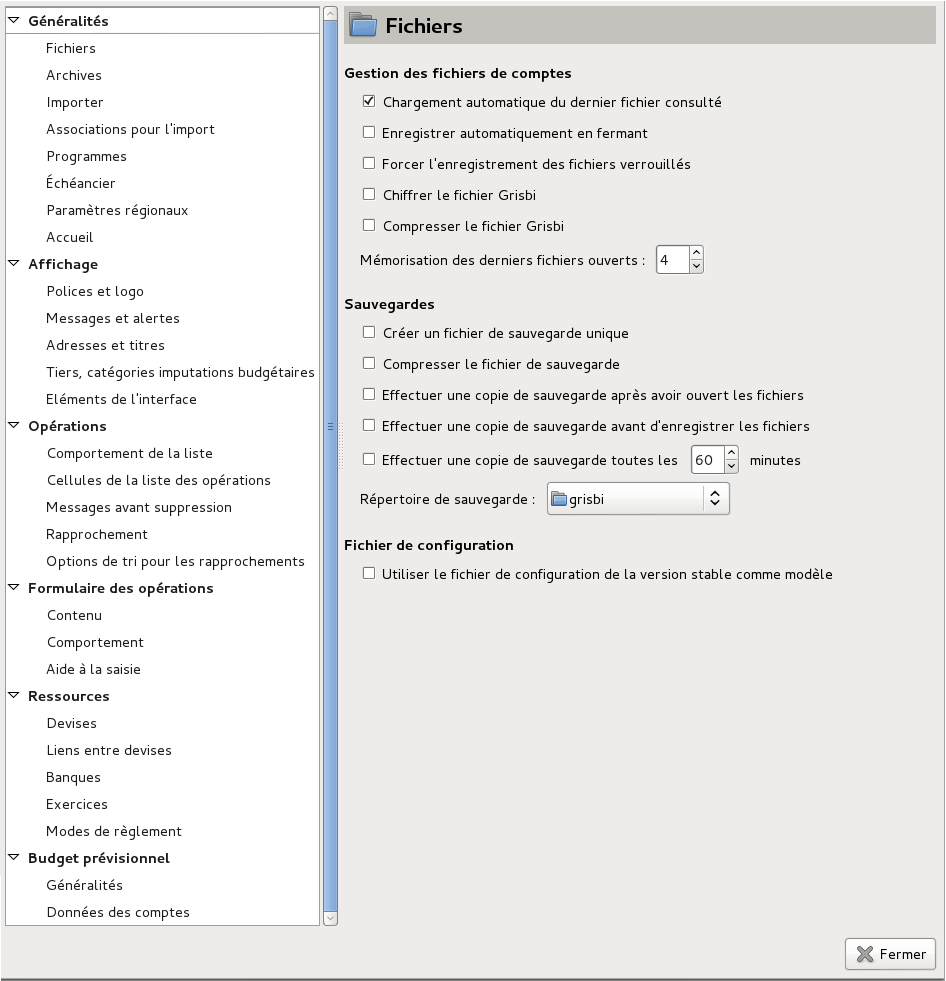
\includegraphics[scale=0.42]{image/screenshot/setup_sections}
\end{center}
\caption{Fenêtre de configuration}
\label{setup-sections-img}
\end{figure}
% image centrée 
\else à droite.
\fi

Il y a vingt-cinq onglets qui sont regroupés en six sections :
\begin{itemize}
	\item \menu{Généralités} ;
	\item \menu{Affichage} ;
	\item \menu{Opérations} ;
	\item \menu{Formulaire des opérations} ;
	\item \menu{Ressources} ;
	\item \menu{Budget prévisionnel}.
\end{itemize}

% espace pour changement de thème
\vspacepdf{5mm}

Vous pouvez sélectionner un autre onglet en cliquant sur son nom, ou en naviguant dans le panneau des onglets avec les touches du clavier   \key{Flèche Haut}, \key{Flèche Bas}, \key{Page Haut}, \key{Page Bas}.

% espace pour changement de thème
\vspacepdf{5mm}

Vous pouvez naviguer entre le panneau des onglets et les différentes options du panneau des réglages avec les touches \key{Tabulation}, \key{Flèche Haut}, \key{Flèche Bas}, \key{Flèche Gauche} et \key{Flèche Droit}.

% espace pour changement de thème
\vspacepdf{5mm}


\subparagraph{Fichier de configuration :\label{setup-conffile}}


Grisbi dispose d'un fichier de configuration appelé grisbi.conf, qui se trouve dans l'arborescence du système d'exploitation ; ce chemin est indiqué automatiquement dans le menu \menu{Éditer -Préférences}, voir la section \vref{setup-general-various-preferences}, \menu{Paramètres Divers}.

% espace pour changement de thème
\vspacepdf{5mm}

\textbf{Note} : dans toutes les fenêtres de configuration, les libellés en bleu, qui sont associés à des cases à cocher, se retrouvent dans le fichier grisbi.conf ; de ce fait il est inutile, et déconseillé, de faire des modifications manuelles dans ce fichier.

% espace avant Attention ou Note  : 5 mm
\vspacepdf{5mm}

\textbf{Note} : à partir de la version 2.xx de Grisbi, la possibilité de configurer certains paramètres de Grisbi en utilisant dconf-editor (Gsettings) dans les systèmes avec GNU/Linux a été supprimée, car cela posait des problèmes avec d'autres systèmes d'exploitation.


\section{Généralités\label{setup-general}}


\subsection{Fichiers\label{setup-general-files}}

Cet onglet définit la façon dont Grisbi utilise vos fichiers \ifIllustration de comptes\refimage{setup-files-img}.

% image centrée 
\begin{figure}[htbp]
\begin{center}
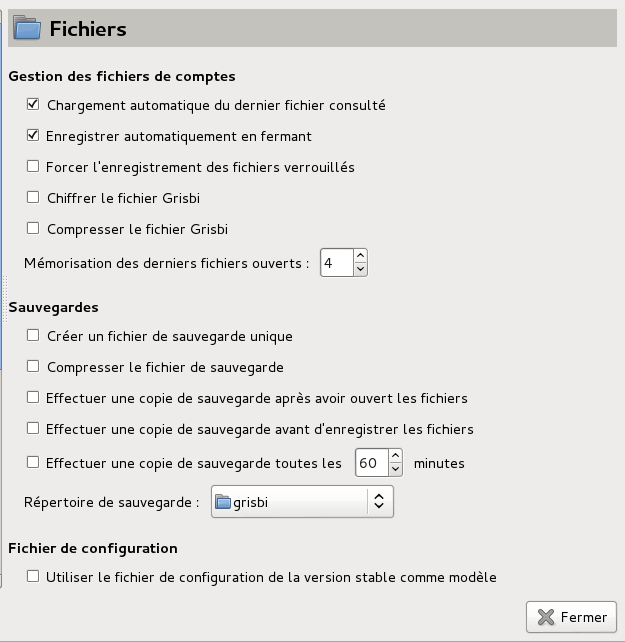
\includegraphics[scale=0.5]{image/screenshot/setup_files}
\end{center}
\caption{Gestion des fichiers de comptes et des sauvegardes}
\label{setup-files-img}
\end{figure}
% image centrée 
\else de comptes.
\fi


\subparagraph{Gestion des fichiers de comptes :\label{setup-general-files-manage}}

Vous pouvez y définir :

\begin{itemize}
	\item \menu{Chargement automatique du dernier fichier consulté} ;
	\item \menu{Enregistrer automatiquement en fermant} : si vous ne cochez pas cette option, lors de la fermeture du fichier ou de l'application ; par défaut, Grisbi n'enregistre pas automatiquement le fichier s'il a été modifié et vous demande si vous voulez l'enregistrer ;
	\item \menu{Forcer l'enregistrement des fichiers verrouillés} : Grisbi permettant à plusieurs utilisateurs d'avoir accès au même fichier de comptes, le fichier en cours d'utilisation est verrouillé en écriture pour les autres utilisateurs qui voudraient l'utiliser en même temps ; mais vous pouvez vouloir forcer l'enregistrement par ces utilisateurs, ou ne vouloir l'enregistrer que si le fichier n'est pas en cours d'utilisation par un autre ; par défaut, l'enregistrement est forcé ;
	\item \menu{Chiffrer le fichier Grisbi} : le \indexword{\gls{chiffrement} du fichier de comptes}\index{fichier de comptes !chiffrement} permet de ne le lire et le modifier que si vous connaissez le mot de passe ; par défaut, il n'est pas chiffré ;
	%saut de ligne pour Note suivante à la ligne en html 

	\strong{Attention} : il n'existe \emph{aucune} méthode pour récupérer un fichier chiffré dont on a perdu le mot de passe.
	%saut de ligne pour Note suivante à la ligne en html

	\strong{Attention} : pour une raison inconnue, l'utilisation de cette fonction de Grisbi sous Windows peut rendre le fichier de comptes totalement inutilisable ; il est donc recommandé de faire des sauvegardes très souvent, ou mieux encore, de ne pas l'utiliser : son utilisation est à vos risques et périls ;
	\item \menu{Compresser le fichier Grisbi} : la \indexword{compression du fichier de comptes} \index{fichier de comptes !compression} permet d'avoir un fichier moins volumineux ; dans ce cas, il ne sera plus lisible directement avec un éditeur de texte ; par défaut, il est compressé, et cette compression est faite au format \file{.\gls{GZ}} ;
	\item \menu{Mémorisation des derniers fichiers ouverts} : réglage, par les boutons \menu{+} et \menu{-}, du nombre des derniers fichiers ouverts, accessibles par le menu \menu{Fichier - Derniers fichiers}.
\end{itemize}

% espace avant Attention ou Note  : 5 mm
\vspacepdf{5mm}
\textbf{Note} : il est conseillé de sélectionner l'option  \menu{ Enregistrer automatiquement en fermant} : les modifications sont sauvegardées à la fermeture de Grisbi sans rien demander à l'utilisateur.


\subparagraph{Sauvegardes :\label{setup-general-files-backup}}

Vous pouvez y définir :

\begin{itemize}
	\item \menu{Créer un fichier de sauvegarde unique} : ce fichier de sauvegarde automatique sera créé par défaut à la racine de votre répertoire personnel, avec une extension automatique du nom de fichier ; par défaut, Grisbi fait plutôt des sauvegardes automatiques à intervalles réguliers ;
	\item \menu{Compresser le fichier de sauvegarde} : par défaut, il n'est pas compressé ;
	\item \menu{Effectuer une copie de sauvegarde après avoir ouvert les fichiers} : dans ce cas, vous indiquerez plus bas un répertoire de sauvegarde ; par défaut, il n'y a pas de sauvegarde automatique après l'ouverture du fichier de comptes ;
	\item \menu{Effectuer une copie de sauvegarde avant d'enregistrer les fichiers} : dans ce cas, vous indiquerez plus bas un répertoire de sauvegarde ; par défaut, il y a une sauvegarde automatique avant l'enregistrement du fichier de comptes ;
	\item \menu{Effectuer une copie de sauvegarde toutes les \ldots{ } minutes} : réglage de l'intervalle entre deux sauvegardes automatiques, en minutes,  par les boutons \menu{+} et \menu{-}  ;
	\item \menu{Supprimer les sauvegardes antérieures à \ldots{ } mois} : réglage de la durée de conservation des sauvegardes automatiques, en mois,  par les boutons \menu{+} et \menu{-}  ;
	\item \menu{Répertoire de sauvegarde} : la liste déroulante permet d'ouvrir différents volumes de stockage, et le choix \menu{Autre} ouvre un gestionnaire de fichiers qui permet d'identifier le chemin du répertoire actuel, et de naviguer dans le système de fichiers pour définir le répertoire de sauvegarde.
\end{itemize}

% espace avant Attention ou Note  : 5 mm
\vspacepdf{5mm}
\textbf{Note} : il est conseillé de sélectionner l'option \menu{ Effectuer une copie de sauvegarde avant d'enregistrer les fichiers} : Grisbi sauvegarde l'ancien fichier avant de faire un enregistrement des dernières modifications.

% espace avant Attention ou Note  : 5 mm
\vspacepdf{5mm}
\strong{Attention} : d'une manière générale, il est déconseillé d'avoir des accents ou des espaces dans les noms des répertoires et fichiers utilisés par Grisbi. Si c'est le cas, renommez-les maintenant. Par exemple, les espaces peuvent être remplacées par des tirets bas (\_). 

\ifIllustration
\else
% saut de page pour titre solidaire
\newpage
\fi


\subsection{Archives\label{setup-general-archives}}

Cet onglet sert à gérer les archives existantes et l'automatisation \ifIllustration de l'archivage\refimage{setup-history-img}.
% image centrée 
\begin{figure}[htb]
\begin{center}
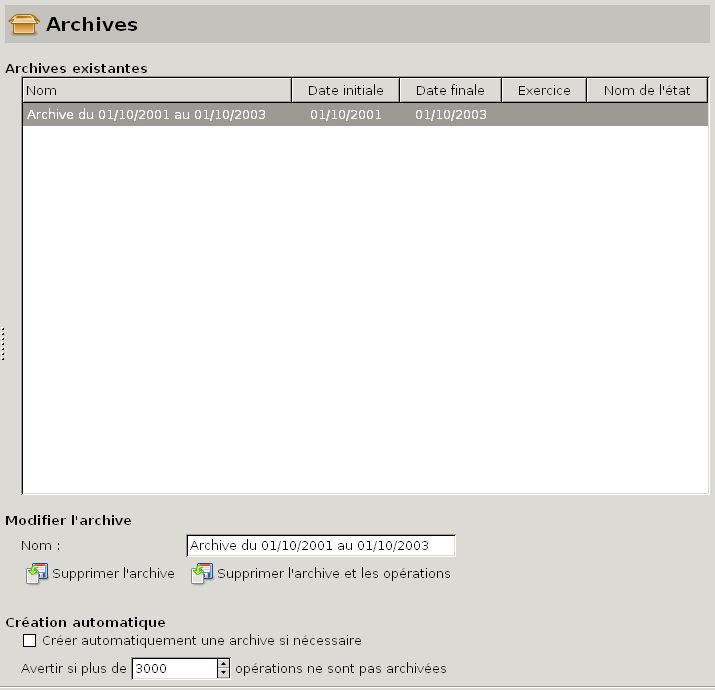
\includegraphics[scale=0.50]{image/screenshot/setup_history}
\end{center}
\caption{Gestion des archives}
\label{setup-history-img}
\end{figure}
% image centrée 
\else de l'archivage.
\fi


\subparagraph{Archives existantes :\label{setup-general-archives-existing}}

Le tableau affiche la \indexword{liste des archives}\index{archive !liste} faites précédemment, avec les informations relatives au mode de sélection des opérations utilisé pour la création de l'archive :

\begin{itemize}
	\item le nom de l'archive ;
	\item si les opérations ont été sélectionnées par date : les dates initiale et finale de l'archive ;
	\item si les opérations ont été sélectionnées par exercice : l'année de l'exercice ;	
	\item si les opérations ont été sélectionnées par un état : le nom de cet état.
	\end{itemize}	

% espace pour changement de thème
\vspacepdf{5mm}
Sous ce tableau, vous pouvez trier ou non les archives en cochant la case \menu{Trier les archives par dates décroissantes}.



\subparagraph{Modifier l'archive :\label{setup-general-archives-remove}}

Si vous sélectionnez une ligne d'archive par un clic dans le tableau, son nom apparaît dans le champ libellé \menu{Nom}, et les deux boutons de \indexword{suppression d'archive}\index{archive ! suppression} \menu{Supprimer l'archive} et \menu{Supprimer l'archive et les opérations} deviennent actifs ; vous pouvez alors :

\begin{itemize}
	\item dans le champ \menu{Nom} : modifier le nom de l'archive ;	
	\item par le bouton \menu{Supprimer l'archive} : par un clic, vous supprimez le statut \emph{archive} des opérations appartenant à l'archive sélectionnée ; ces opérations seront donc à nouveau visibles dans la liste des opérations ;  une fenêtre d'avertissement et de validation s'affiche et vous pouvez soit valider, soit annuler cette action ; cette opération est réversible, en recréant la même archive ;
	\item par le bouton \menu{Supprimer l'archive et les opérations} : par un clic, vous  supprimez du fichier de comptes de Grisbi l'archive sélectionnée \emph{et toutes les opérations contenues dans celle-ci} ; une fenêtre d'avertissement et de validation s'affiche et vous pouvez soit valider, soit annuler cette action ; cette \indexword{opération est irréversible}\index{opération !irréversible}, et il est vivement conseillé d'exporter auparavant l'archive vers un fichier au format \gls{GSB}, \gls{QIF} ou \gls{CSV} (voir \menu{Fichier - Exporter une archive vers un fichier GSB/ QIF/CSV/...}

% espace après Attention ou Note  : 5 mm
\vspacepdf{5mm}
\strong{Attention} :  si vous choisissez cette dernière fonction, il n'y aura pas d'autre avertissement, et l'archive sera supprimée \emph{IMMÉDIATEMENT} ainsi que toutes ses opérations. Cette suppression est irréversible !
\end{itemize}


\subparagraph{Création automatique :\label{setup-general-archives-create}}

Lorsqu'un certain nombre d'opérations enregistrées est atteint, Grisbi peut d'une part afficher un  \indexword{avertissement}\index{archive !avertissement} que cette quantité d'opérations n'a pas été encore archivée, d'autre part lancer automatiquement la \indexword{création d'une archive}\index{archive !création automatique}.

En cliquant sur la case libellée \menu{Créer automatiquement une archive si nécessaire}, vous validez cette fonction d'archivage automatique.

Avec le libellé \menu{Avertir si plus de \ldots{ } opérations ne sont pas archivées}, vous pouvez définir ce nombre d'opérations. La valeur par défaut est 3000, mais vous pouvez la modifier par les boutons \menu{+} et \menu{-}.


\subsection{Importer\label{setup-general-import}}

% image centrée 
L'onglet \menu{Importer} sert à configurer certains \ifIllustration paramètres d'importation de données\refimage{setup-import-img}.
\begin{figure}[htbp]
\begin{center}
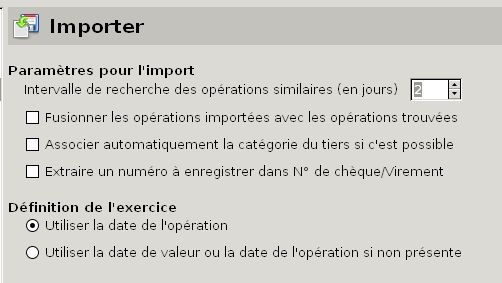
\includegraphics[scale=0.5]{image/screenshot/setup_import}
\end{center}
\caption{Paramètres d'importation}
\label{setup-import-img}
\end{figure}
% image centrée 
\else paramètres d'importation de données.
\fi

Il affiche deux sous-onglets : \menu{Importation des fichiers} et \menu{Associations pour l'importation}

\subsubsection{Importation des fichiers\label{setup-general-import-files}} 

%\subsubsection{Importation des fichiers\label{setup-general-import-parameters}}


Quand vous importez un compte, Grisbi vérifie, pour chaque opération de ce compte, si elle existe déjà dans votre fichier de comptes : si l'opération importée comporte un identifiant bancaire (ce qui est généralement le cas), il commence par chercher une opération qui a le même identifiant. S'il ne trouve pas, il va chercher une opération du même montant et à une date proche.

% espace pour changement de thème
\vspacepdf{5mm}

\subparagraph{Paramètres pour l'import :\label{setup-general-import-files-parameters}}

%\subsubsection{Paramètres pour l'import\label{setup-general-import-parameters}}

Le champ de libellé \menu{Intervalle de recherche des opérations similaires} permet de définir, par les boutons \menu{+} et \menu{-}, sur combien de jours avant et après la date de l'opération importée Grisbi va faire cette recherche. Ainsi, si le réglage est de 5 (sa valeur par défaut est 2), pour une opération datée du 10 du mois, des opérations similaires seront recherchées entre le 5 et le 15.

Vous pouvez faire les choix suivants :

\begin{itemize}
	\item \menu{Fusionner les opérations importées avec les opérations trouvées} : fusionne les opérations importées à partir d'un fichier au format \gls{OFX} avec les opérations planifiées trouvées dans l'intervalle de temps défini ci-dessus ;
	\item \menu{Associer automatiquement la catégorie au tiers si c'est possible} : associe au tiers la catégorie et l'imputation budgétaire de la dernière opération ayant eu le même tiers, sauf pour les chèques ;
	\item \menu{Extraire un numéro à enregistrer dans \No chèque/virement} : récupère un numéro contenu dans le tiers pour le sauvegarder dans le champ \menu{\No chèque/virement} ;
	\item \menu{Sauvegarder le tiers dans les remarques} : recopie le libellé du tiers dans les remarques ; c'est une précaution qui peut faciliter les opérations d'importation.
	
\end{itemize}


\subparagraph{Import des fichiers CSV :\label{setup-general-import-files-CSV}}

Vous pouvez \menu{Forcer la date de valeur, si elle n'existe pas, par la date de l'opération}.


\subparagraph{Import des fichiers QIF :\label{setup-general-import-files-QIF}}

Vous pouvez faire les choix suivants :

\begin{itemize}
	\item \menu{Ne pas importer les catégories} ;
	\item \menu{Si possible, utiliser le champ « N » pour définir le mode de paiement} : il s'agit d'un ajout pour l'importation des fichiers QIF spécifiques de la banque Société Générale ;
		
\end{itemize}


\subparagraph{Définition de l'exercice :\label{setup-general-import-files-financialyear}}

Vous pouvez définir quelle type de date sera utilisée pour l'attribution de l'\indexword{exercice}\index{exercice !définition} à chaque opération importée, en choisissant entre les boutons :

\begin{itemize}
	\item \menu{Utiliser la date de l'opération} : c'est le choix par défaut ;     
	\item \menu{Utiliser la date de valeur ou la date de l'opération si non présente}.
\end{itemize}






\subsubsection{Associations pour l'importation\label{setup-general-importlinks}}

\ifIllustration
% image entourée par un paragraphe ( picins)
% pas de référence à l'illustration car erreur de numéro de figure avec picins.
\pichskip{8mm}
% supprimé car en html les figures entourées ne sont pas numérotées, et la numérotation des figures centrées décalée par rapport au pdf
%\piccaption{Associations pour l'importation}
\label{setup-importLinks-img}
\parpic[r]{\includegraphics[scale=0.5]{image/screenshot/setup_importlinks}}
\picskip{18}
% image entourée par un paragraphe ( picins)
\fi
\noindent Lorsque vous importez un fichier, vous pouvez établir une association entre une \indexword{chaîne de caractères}\index{chaîne de caractères} de ce fichier et un tiers déjà existant dans votre fichier de comptes. Par exemple, tous les libellés \gls{QIF} contenant \og loyer \fg{} peuvent être associés à un tiers qui peut, par exemple, représenter votre propriétaire. Cela permet de définir automatiquement des tiers à partir d'informations pour lesquelles vous savez qu'elles ont un rapport.

%\newlinepdf

\ifIllustration
% espace après légende  : 10 mm
\vspacepdf{15mm}
\fi

\subparagraph{Associations pour l'import :\label{setup-general-importlinks-array}}

Le tableau affiche les différentes associations tiers-chaîne de caractères que vous avez créées, et deux boutons \menu{Ajouter} et \menu{Enlever}. 


\subparagraph{Détails des associations :\label{setup-general-importlinks-details}}
%% espace pour changement de thème
%\vspacepdf{5mm}
La section \menu{Détails des associations} affiche un champ de saisie et une liste déroulante pour le \menu{Nom du tiers}, et un champ de saisie pour la \menu{Chaîne recherchée} : cela permet d'afficher les paramètres de l'association pour l'import\index{import !paramétrage} sélectionnée dans le tableau, ou de créer ou modifier une association.

% espace pour changement de thème
\vspacepdf{5mm}

Vous disposez aussi de deux boutons \menu{Ignorer la casse}, pour trouver une chaîne contenant à la fois des caractères majuscules et minuscules, et \menu{Utiliser les expressions régulières}.

% espace pour changement de thème
\vspacepdf{5mm}
CASSE et expressions régulières : AJOUTER DANS L'INDEX ET DANS LE GLOSSAIRE



\ifIllustration
% espace après image entourée
\vspacehevea{20mm}
\fi

% espace pour changement de thème
\vspacepdf{5mm}

Pour ajouter une association, procédez comme suit :
\begin{enumerate}
	\item saisissez un nom dans le champ \menu{Nom du tiers} ; Grisbi vous propose le complètement automatique d'après les tiers connus ; ou bien sélectionnez un tiers dans la liste déroulante, indiquée par un petit triangle noir à droite ;
	
			\textbf{Note} : ces triangles peuvent être remplacés, en fonction du thème de l'environnement de bureau ou du gestionnaire de fenêtres que vous utilisez, par d'autres caractères tels que +, -, >, <, etc.
	\item saisissez une chaîne de caractères à rechercher dans le champ \menu{Chaîne recherchée} ; vous pouvez utiliser le caractère \og \% \fg{} comme joker, par exemple \og Carte Visa\% \fg{}, \og\%Tresor Public\% \fg{} ou \og VIR \% BANQUE \fg{} ;
	\item cliquez sur le bouton \menu{Ajouter} ; l'association s'affiche dans le tableau.
\end{enumerate}

\vspacepdf{5mm}

Pour modifier une association, procédez comme suit :
\begin{itemize}
	\item modification du tiers :
		\begin{enumerate}
			\item sélectionnez l'association dans le tableau par un clic de souris : ses paramètres apparaissent dans la section \menu{Détails des associations},
			\item dans cette section, modifiez le tiers dans le champ de saisie libellé \menu{Nom du tiers}, ou grâce à la liste déroulante à sa droite, indiquée par un petit triangle noir à droite ;	
	%saut de ligne pour Note suivante à la ligne en html 

			\textbf{Note} : ces triangles peuvent être remplacés, en fonction du thème de l'environnement de bureau ou du gestionnaire de fenêtres que vous utilisez, par d'autres caractères tels que +, -, >, <, etc.
		\end{enumerate}		
	\item modification de la chaîne recherchée :		
		\begin{enumerate}
			\item dans la colonne \menu{Chaîne recherchée} du tableau, cliquez sur la ligne de l’association : cela met son champ \menu{Chaîne recherchée} en mode édition,
			\item modifiez-la, puis validez par la touche \key{Entrée} ; le champ \menu{Chaîne recherchée} de cette association est mis à jour.	
		\end{enumerate}
\end{itemize} 
 
\ifIllustration
% espace pour changement de thème
\vspacepdf{5mm}
\fi 
 
Pour supprimer une association, procédez comme suit :
\begin{enumerate}
	\item sélectionnez-la dans le tableau par un clic de souris ;
	\item cliquez sur le bouton \menu{Enlever} ; l'association disparaît du tableau.
\end{enumerate}





\subsection{Paramètres divers\label{setup-general-various}}

Cet onglet permet de gérer plusieurs aspects de l'utilisation de Grisbi. 


\subsubsection{Généralités\label{setup-general-various-general}}


\subparagraph{Navigateur Web :\label{setup-general-various-general-browser}}

Cette section permet de définir le navigateur Web qui sera lancé par les différents choix du menu \menu{Aide}, et qui affichera directement les contenus au format \gls{HTML}. 

Le champ \indexword{navigateur Web}\index{navigateur Web} permet de spécifier ce programme. La commande \cmd{xdg-open}, présente par défaut et reconnue par tous les bons systèmes d'exploitation (!), lance votre navigateur par défaut.

Mais vous pouvez aussi saisir la commande qui lance un autre navigateur, par exemple \cmd{firefox} ou bien, si vous voulez un affichage ultra-rapide, un navigateur ultra-léger comme Dillo ou Midori (commande \cmd{dillo} ou \cmd{midori}), voir la section \vref{introduction-manual-readers}, \menu{Logiciels de lecture}. Le navigateur affiche alors la page HTML demandée dans le menu \menu{Aide} : soit le \menu{Manuel}, le document \menu{Démarrage rapide}, le \menu{Site Web de Grisbi} ou le site \menu{Signaler une anomalie}.


\subparagraph{Affichage de l'aide :\label{setup-general-various-general-display}}

Vous avez le choix d'afficher l'aide soit au format \gls{HTML}, grâce au navigateur défini ci-dessus, ou au format \gls{PDF}, grâce à votre lecteur PDF par défaut ; ceux-ci sont normalement définis dans la configuration de votre interface graphique (Windows, Mac OSX, ou bien pour les systèmes Linux : Gnome, KDE, XFCE, Enligthenment ou tout autre gestionnaire de fenêtres). 


VÉRIFIER QUE NAVIGATEUR ET LECTEUR PDF SONT DANS LE GLOSSAIRE ET L'INDEX



\ifIllustration
% image entourée par un paragraphe ( picins)
% pas de référence à l'illustration car erreur de numéro de figure avec picins.
\pichskip{7mm}
% supprimé car en html les figures entourées ne sont pas numérotées, et la numérotation des figures centrées décalée par rapport au pdf
%\piccaption{Lancement de programmes}
\label{setup-programs-img}
\parpic[l]{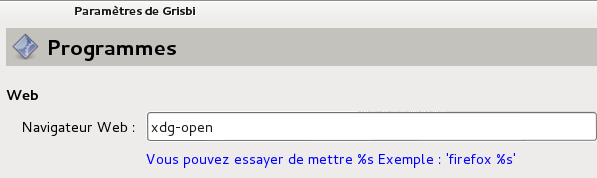
\includegraphics[scale=0.5]{image/screenshot/setup_programs}}
%\picskip{8} ne marche plus, superpose le texte et l'image
% image entourée par un paragraphe ( picins)
\fi


%\newlinepdf


% espace avant Attention ou Note  : 10 mm
%\vspacepdf{5mm}
%\textbf{Note} : dans cette commande, vous devrez peut-être indiquer aussi le chemin d'accès complet à la commande.

\ifIllustration
% espace après image entourée
\vspacehevea{2mm}
\fi

%\vspacepdf{5mm}
%\textbf{Note} : cela peut fonctionner de saisir une commande pour lancer l'affichage du manuel en pdf, par ex. \cmd{evince chemin/grisbi-manuel-img-xxx.pdf} avec son chemin ; il se peut que cela affiche aussi une erreur peu importante, mais si vous préférez ce format \dots



\subparagraph{Paramètres des préférences :\label{setup-general-various-general-preferences}}

Cette section affiche le chemin complet du fichier de configuration de Grisbi dans votre système (voir le chapitre \vref{setup-conffile}, \menu{Fichier de configuration}).


Le bouton \menu{Réinitialisation de la fenêtre des préférences} permet de réinitialiser les dimensions de cette fenêtre en fonction de l'écran utilisé. À PRÉCISER


\subsubsection{Échéancier\label{setup-general-various-planned}}

L'échéancier (voir le chapitre \vref{plannedtransactions}, \menu{Échéancier}) vous permet de définir des opérations à exécution manuelle ou automatique. Pour les opérations automatiques, il vous signifiera une \indexword{alerte d'opération planifiée}\index{alerte !opération planifiée} à l'approche de l'échéance de chaque l'opération, par un message qui s'affiche dans la page d'accueil. L'alerte et l'exécution sont normalement simultanées.

\subparagraph{Options de lancement des opérations planifiées :\label{setup-general-various-planned-options}}

Vous devrez choisir entre l'une des deux options :
% espace avant image 5mm
\vspacepdf{3mm}

\begin{itemize}
	% image entourée par une liste (picins)
	% pas de référence à l'illustration car erreur de numéro de figure avec picins.
	\ifIllustration
	% supprimé car en html les figures entourées ne sont pas numérotées, et la numérotation des figures centrées décalée par rapport au pdf
	%\piccaption{Alertes de l'échéancier}
	\label{setup-plannedtransactions-img}
	\parpic[l]{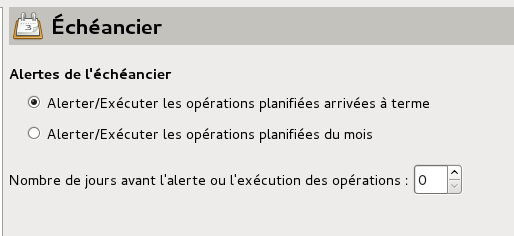
\includegraphics[scale=0.5]{image/screenshot/setup_plannedtransactions}}
	% image entourée par une liste 
	\fi
	\item \menu{Alerter/Exécuter les opérations planifiées arrivées à terme} : le message n'apparaît qu'à la date où l'opération est échue, c'est le choix par défaut ; mais vous pouvez spécifier un \menu{Nombre de jours avant l'alerte et l'exécution automatique des opérations} en l'ajustant avec les boutons \menu{+} et \menu{-} ;
	
	% espace avant image 5mm
	\vspacepdf{3mm}
	À VOIR AVEC ALAIN : message d'Alain du 24/02, et réenvoyé à Pierre pour avoir son avis (03/03/2021 à 16:54). En attente de réponse.
	
	
	% espace avant image 5mm
	\vspacepdf{3mm}
	
	
	\item \menu{Alerter/Exécuter les opérations planifiées du mois} : tous les messages relatifs aux  opérations à échoir durant le mois  apparaissent dès le 1\up{er} jour du mois ; mais vous pouvez modifier ce jour en sélectionnant \menu{Jour de lancement des opérations exécutées mensuellement} et en ajustant le jour du mois avec les boutons \menu{+} et \menu{-} ; cette option permet d'anticiper l'alerte et l'exécution des opérations planifiées du mois suivant ; par exemple, si l'opération planifiée se situe au mois de mai, vous pourrez anticiper l'alerte et l'exécution au 25 avril en choisissant « 25 » avec les boutons \menu{+} et \menu{-}.
\end{itemize}

% espace pour changement de thème
\vspacepdf{5mm}
	
L'option \menu{Fixer la date pour les transactions planifiées les 28, 29 et 30 et 31 du mois} permet de définir le jour de de l'opération si elle existe ; cela permet de ne pas avoir de conflit si la date n'existe pas (fins de mois ou années bissextiles) ; par exemple, si vous avez une opération planifiée au 31 mai, le mois suivant l'opération sera anticipée au 30 juin.


\ifIllustration
% espace après légende  : 10 mm
\vspacepdf{12mm}
\fi



\ifIllustration
% espace après image entourée
\vspacehevea{15mm}
\fi
%
%



\subparagraph{Autres Options :\label{setup-general-various-planned-otherOptions}}

Lorsque vous ouvrez l'onglet \menu{Échéancier} du panneau de navigation, la liste des opérations planifiées et le formulaire de saisie des opérations  s'affichent dans le panneau des détails ; il est possible de définir le compte qui s'affichera par défaut dans le formulaire de saisie des opérations. Ce compte devrait être le compte le plus utilisé pour les opérations planifiées ; pour cela, cochez la case \menu{Utiliser un compte par défaut dans le planificateur}, et choisissez-le dans la liste déroulante à sa droite.

% espace pour changement de thème
\vspacepdf{5mm}

Vous pouvez aussi définir l’opération qui sera sélectionnée par défaut dans la liste des opérations : elle sera surlignée en rose{\couleur} : cochez la case \menu{première} ou \menu{dernière} opération de la liste. La prise en compte du changement prendra effet au redémarrage de Grisbi.



\subsubsection{Paramètres régionaux\label{setup-general-various-regional}}


\subparagraph{Choisir la langue :}\index{langue !séparateur}\label{setup-general-various-regional-langue} Choisissez dans la liste déroulante la langue que va utiliser Grisbi.

\subparagraph{Choisir le format de la date :}\index{date !séparateur}\index{séparateur !date}\index{date !format}\label{setup-general-localisation-date}

Grisbi vous laisse le choix dans le format de la date. Vous pouvez choisir son format entre les boutons :
\begin{itemize}
	\item \menu{dd/mm/yy} : affichage du jour, du mois et de l'année ; c'est le format utilisé dans les pays francophones et au Royaume-Uni, et c'est le format par défaut ;    
	\item \menu{mm/dd/yy} : affichage du mois, du jour et de l'année ; c'est le format utilisé aux États-Unis ;
	\item \menu{yyyy.mm.dd} : affichage du jour, du mois et de l'année ; c'est le format utilisé au Canada.
\end{itemize}

% espace pour changement de thème
\vspacepdf{5mm}

%Pour d'autres pays, rendez-vous sur la page « Date » de \lang{Wikipédia}\footnote{\urlWikipediaDate{}}.



\subparagraph{Choisir le séparateur décimal et le séparateur des milliers :}\index{séparateur !milliers\label{setup-general-localisation-numbers}}

Vous pouvez choisir dans les deux listes déroulantes :
\begin{itemize}
	\item le \indexword{séparateur décimal} ; la virgule est le séparateur utilisé dans les pays francophones, et c'est le séparateur par défaut ;    
	\item le \indexword{séparateur des milliers} ; l'espace est le séparateur utilisé dans les pays francophones, et c'est le séparateur par défaut.
\end{itemize}


\subsection{Accueil\label{setup-general-home}}

L'onglet \menu{Configuration de la page d'accueil} permet de configurer trois aspects \ifIllustration de la page d'accueil\refimage{setup-home-img}.
%image centrée
\begin{figure}[ht]
\begin{center}
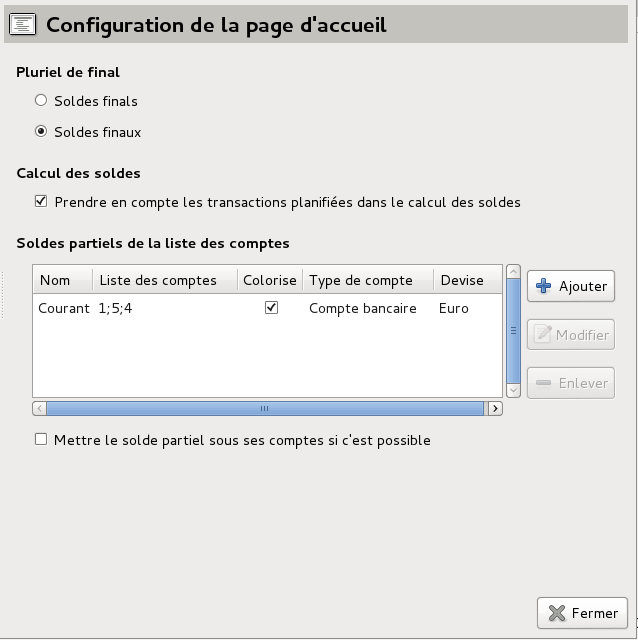
\includegraphics[scale=0.5]{image/screenshot/setup_home}
\end{center}
\caption{Configuration de la page d'accueil}
\label{setup-home-img}
\end{figure}
%image centrée
\else de la page d'accueil.
\fi


\subparagraph{Pluriel de final :\label{setup-general-home-final}}

Ce \indexword{pluriel du mot \og final \fg{}} \index{pluriel de final}apparaît notamment dans la page d'accueil. Vous pouvez choisir le pluriel de \og Solde final \fg{}, entre \menu{Soldes finals} (choix par défaut) et \menu{Soldes finaux}. En français, l'emploi de l'un ou l'autre est possible, c'est donc à votre convenance. 


\subparagraph{Calcul des soldes :\label{setup-general-home-balance}}

Vous pouvez choisir de \menu{Prendre en compte les transactions planifiées dans le calcul des soldes}\index{solde !opérations planifiées} en cochant la case correspondante : c'est le choix par défaut.


\subparagraph{Position dans la liste des soldes partiels :\label{setup-general-home-partBalance}}

La page d'accueil affiche le solde de chaque compte créé dans Grisbi (voir la section \vref{home-details-homepage}, \menu{Affichage de la page d'accueil}), ainsi que le solde final de tous les comptes. Vous pouvez aussi lui faire afficher les soldes de plusieurs comptes, groupés par vous-mêmes en \indexword{groupes de comptes}\index{groupe de comptes}. Ces \indexword{soldes partiels}\index{solde !partiel} seront affichés en-dessous des \indexword{soldes des comptes}\index{solde !comptes}, et leur ordre peut être ajusté à votre convenance, ainsi que leur couleur (voir la section \vref{setup-display-logo-CSS}, \menu{Règles CSS}).

% espace pour changement de thème
\vspacepdf{5mm}
Le tableau affiche les groupes de comptes\index{groupe de comptes !solde partiel} et leurs paramètres : \menu{Nom}, \menu{Liste des comptes}, \menu{Colorise}, \menu{Type de compte}, \menu{Devise}.

% espace pour changement de thème
\vspacepdf{5mm}
Vous pouvez ajuster l'ordre d'\indexword{affichage des soldes partiels}\index{affichage !soldes partiels} dans la page d'accueil de plusieurs manières :

\begin{itemize}
	\item en cochant ou non la case \menu{Placer si possible le solde partiel sous ses comptes}, qui se trouve au-dessus du tableau ;
	\item en modifiant l'ordre des numéros des comptes dans la Liste des comptes du tableau ; chaque compte a un numéro qui est affiché dans l'onglet \menu{Propriétés} du compte (voir la section \vref{accounts-properties}, \menu{Propriétés d'un compte})
	\item en sélectionnant la ligne du groupe dans le tableau et en déplaçant la sélection dans la liste par glisser-déposer.
\end{itemize}

\ifIllustration
% saut de page pour phrase solidaire
\newpage
\fi

% espace pour changement de thème
\vspacepdf{5mm}

Pour \indexword{ajouter un groupe de comptes}\index{groupe de comptes !ajouter} dans la liste, procédez comme suit :

\begin{enumerate}
	\item cliquez sur le bouton \menu{Ajouter} ; la fenêtre \menu{Détails des soldes partiels} s'affiche ;
	\item saisissez le nom de votre nouveau groupe de comptes dans le champ \menu{Nom} ;
	\item sélectionnez au moins deux comptes dans la liste \menu{Nom du compte}, en utilisant la sélection multiple avec \key{Ctrl}\key{Clic} ou  \key{Majuscule}\key{Clic} ; 
	\item définissez la position de ce solde partiel dans la page d'accueil dans le champ \menu{Position dans la liste des comptes} avec les boutons \menu{+} et \menu{-} ;
	\item sélectionnez ou non la case \menu{Colorié en rouge, si le solde est négatif}, puis validez par le bouton \menu{Valider} ; vous revenez alors sur la fenêtre \menu{Configuration de la page d'accueil}
 	\item le libellé \menu{Liste des comptes} indique les numéros d'ordre des comptes choisis (ces numéros correspondent à l'ordre de création de chaque compte) ;
	\item le libellé \menu{Position dans la liste des comptes} indique le numéro d'ordre de création du groupe de comptes.
	\item quand il est négatif, le solde s'affiche par défaut en noir{\couleur} ; cochez la case \menu{Colorise} pour qu'il s'affiche en rouge{\couleur} dans ce cas,  puis validez par le bouton \menu{Valider} ;
	\item si les comptes sélectionnés ont des devises différentes, une fenêtre s'ouvre, sélectionnez la devise du solde partiel, puis validez par le bouton \menu{Valider} ;
	\item le tableau \menu{Soldes partiels de la liste des comptes} affiche maintenant la ligne de votre nouveau groupe de comptes. 
\end{enumerate}

% espace pour changement de thème
\vspacepdf{5mm}
Pour \indexword{modifier un groupe de comptes}\index{groupe de comptes !modifier} dans la liste, procédez comme suit :

\begin{enumerate}
	\item sélectionnez un groupe de comptes par un clic sur sa ligne ;
	\item cliquez sur le bouton \menu{Modifier} : la fenêtre \menu{Détail des soldes partiels} s'affiche : les comptes du groupe sont affichés sur fond grisé ;
	\item modifiez le nom de votre groupe de comptes dans le champ \menu{Nom} ;
	\item changez votre sélection de comptes (gardez au moins deux comptes dans la liste), en utilisant la sélection multiple avec \key{Ctrl}\key{Clic} ou \key{Majuscule}\key{Clic} ; 
 	\item le libellé \menu{Liste des comptes} indique les numéros d'ordre modifiés des comptes choisis ;
	\item le libellé \menu{Position dans la liste des comptes} indique le même numéro d'ordre de création du groupe de comptes qu'auparavant.

	\item cochez la case  \menu{Colorié en rouge{\couleur}}, si le solde est négatif, à votre convenance, puis validez par le bouton \menu{Valider} ;
	\item si les comptes sélectionnés ont des devises différentes, une fenêtre s'ouvre, sélectionnez la devise du solde partiel, puis validez par le bouton \menu{Valider} ;
	\item le tableau \menu{Soldes partiels de la liste des comptes} affiche maintenant la ligne de votre nouveau groupe de comptes modifié. 
\end{enumerate}

% espace pour changement de thème
\vspacepdf{5mm}

Pour \indexword{supprimer un groupe de comptes}\index{groupe de comptes !supprimer} dans la liste, procédez comme suit :

\begin{enumerate}
	\item sélectionnez un groupe de comptes par un clic sur sa ligne ;
	\item cliquez sur le bouton \menu{Effacer} ; le groupe de comptes sélectionné disparaît de la liste.
\end{enumerate}

% saut de page pour titre solidaire
\newpage


\section{Affichage\label{setup-display}}


\subsection{Polices et logo\label{setup-display-logo}}

Vous pouvez changer le logo de Grisbi, la police de caractères utilisée pour les opérations, le thème, les règles CSS (couleurs) et la taille globale de la police de caractères \ifIllustration  \refimage{setup-fonts-logo-img}.
% image centrée
\begin{figure}[htbp]
\begin{center}
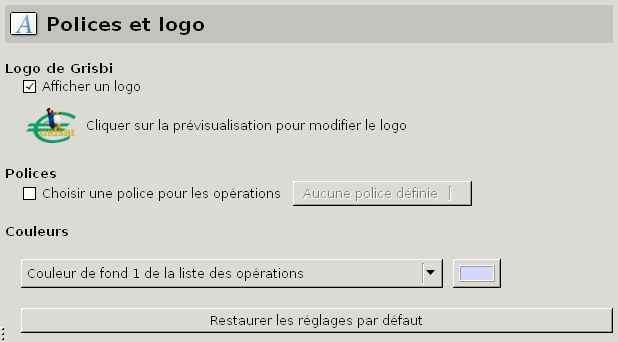
\includegraphics[scale=0.5]{image/screenshot/setup_fonts_logo}
\end{center}
\caption{Logo de Grisbi, polices de caractères et couleurs}
\label{setup-fonts-logo-img}
\end{figure}
% image centrée
\else certaines couleurs IMAGE À VOIR.
\fi


\subparagraph{Logo de Grisbi :\label{setup-display-logo-icon}}

Vous pouvez afficher ou non un logo dans la page d'accueil de Grisbi en (dé)cochant le bouton \menu{Afficher un logo}. Le logo par défaut est celui qui est affiché en miniature devant le libellé \menu{Cliquez sur la prévisualisation pour modifier le logo} ; vous pouvez en changer à votre convenance. 

% espace avant Attention ou Note  : 5 mm
\vspacepdf{5mm}
Pour changer le logo, procédez comme suit :

\begin{enumerate}
	\item cliquez sur la prévisualisation du logo ;
	\item une fenêtre de gestionnaire de fichiers s'affiche ;
	\item naviguez dans l'arborescence des fichiers pour trouver votre nouveau logo ; ce doit être un fichier avec une extension de format d'image ; puis validez ;
	\item la prévisualisation du nouveau logo s'affiche.
\end{enumerate}

% espace pour changement de thème
\vspacepdf{5mm}
\textbf{Note} : Cette fonction est surtout intéressante pour les trésoriers d'associations (ou d'autres organisations) qui pourront ainsi imprimer des états avec leur propre logo au lieu de celui de Grisbi.

\textbf{Note} : le logo de Grisbi existe en plusieurs formats, dont \gls{PNG}, et \gls{SVG}.

%Voir pour \gls{ICO}
% espace après Attention ou Note  : 5 mm
\vspacepdf{5mm}


\subparagraph{Polices :\label{setup-display-logo-fonts}}

Pour changer la police de caractères utilisée dans Grisbi pour les opérations, procédez comme suit :

\begin{enumerate}
	\item cliquez sur la case \menu{Choisir une police pour les opérations} : cela valide à droite le champ indiquant le nom de la police courante et sa taille ;
	\item cliquez sur ce champ : une fenêtre de choix de police s'affiche ;
	\item sélectionnez la police, le style et la taille puis validez par le bouton \menu{Valider}.
\end{enumerate}

% EN COMMENTAIRE : LA VERSION 1.0
%\subsubsection{Couleurs\label{setup-display-logo-colors}}
%
%Toutes les couleurs accessibles dans la liste déroulante commençant par \menu{Couleur de fond 1 de la liste des opérations} sont modifiables ; pour les modifier,  procédez comme suit :
%
%\begin{enumerate}
%	\item cliquez sur la liste déroulante et choisissez l'une des possibilités proposées ;
%	\item cliquez sur le pavé de choix des couleurs juste à droite : la fenêtre de palette des couleurs s'affiche ;
%	\item sélectionnez la couleur désirée, puis validez par le bouton \menu{Valider}.
%\end{enumerate}
%
%La \menu{Couleur pour l'opération qui donne le solde à aujourd'hui} sert à distinguer le solde du compte quand on a choisi l'option \menu{Exécuter les opérations planifiées du mois} (voir la section \vref{setup-general-planned}, \menu{Échéancier}).
%
%Vous pouvez revenir aux réglages de couleur d'origine en cliquant sur le bouton \menu{Restaurer les réglages par défaut}.
%
%
%\subsection{Messages et alertes\label{setup-display-messages}}
%
%Cet onglet permet d'autoriser ou non l'affichage des messages et des alertes \ifIllustration que vous renvoie Grisbi\refimage{setup-messages-alerts-img}.
%\else que vous renvoie Grisbi.
%\fi
%
%\ifIllustration
%% image centrée 
%\begin{figure}[h!]
%\begin{center}
%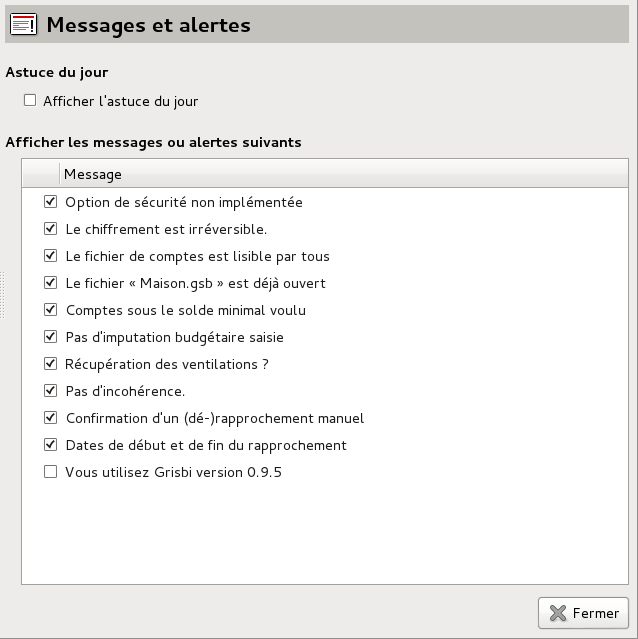
\includegraphics[scale=0.5]{image/screenshot/setup_messages_alerts}
%\end{center}
%\caption{Messages et alertes}
%\label{setup-messages-alerts-img}
%\end{figure}
%% image centrée 
%\fi
% EN COMMENTAIRE : LA VERSION 1.0

\subparagraph{Thème :\label{setup-display-logo-theme}}

Le thème utilisé dans Grisbi est, par défaut, « Adwaita ». Si cela ne vous convient pas, vous pouvez le changer grâce à la liste déroulante de cette section. Les possibilités de changement sont :

\begin{itemize}
	\item Sélection automatique (thème par défaut) ;
	\item Forcer l'utilisation d'un thème clair ;
	\item Forcer l'utilisation d'un thème sombre ;	
	\item Forcer l'utilisation d'un thème léger.
\end{itemize}



\subparagraph{Règles CSS :\label{setup-display-logo-CSS}}

Les règles CSS permettent d'ajuster indépendamment l'aspect des affichages suivants :

\begin{itemize}
	\item Page d'accueil ;
	\item Liste des opérations ;
	\item Prévisions (dans la liste des opérations ;	
	\item Préférences ;
	\item Taille globale de la police de caractères.
\end{itemize}

% espace pour changement de thème
\vspacepdf{5mm}

Pour les 4 premiers affichages, une liste déroulante en-dessous propose différents éléments à modifier, et un clic sur le pavé de couleur à sa droite affiche un nuancier pour en définir la couleur. Pour le dernier, une autre liste déroulante permet de définir la hauteur totale des caractères, globalement sur l'ensemble de Grisbi.

% espace pour changement de thème
\vspacepdf{5mm}

En-dessous de ces listes, le bouton \menu{Retour aux valeurs par défaut} permet d'annuler toutes les modifications faites précédemment. 

% espace avant Attention ou Note  : 5 mm
\vspacepdf{5mm}
\strong{Attention} : Ce bouton supprime complètement le fichier personnalisé des couleurs de Grisbi.



\subsection{Messages et alertes\label{setup-display-messages}}



\subparagraph{Astuce du jour :\label{setup-display-messages-trick}}

Avec la case à cocher \menu{Afficher l'astuce du jour}, vous autorisez ou non  l'affichage de la fenêtre de l'astuce du jour\index{astuce du jour} dans la page d'accueil, à chaque démarrage de Grisbi (par défaut, elle ne sera pas affichée). De toutes manières, cette fenêtre peut aussi être affichée à tout moment, en sélectionnant le menu \menu{Aide - Astuce du jour}.


\subparagraph{Afficher les messages ou alertes suivants :\label{setup-display-messages-alerts}}

En (dé)cochant la case correspondante, vous pouvez autoriser ou non l'affichage des \indexword{messages d'alerte}\index{alerte !messages}\index{messages !alerte} suivants  :

\begin{itemize}
	\item \menu{Le fichier \file{nom\_de\_votre\_fichier.gsb} est déjà ouvert} ;
	\item \menu{Le fichier de comptes est lisible par tous} ;
	\item \menu{Vous utilisez Grisbi version \emph{numéro-de-version-de-Grisbi}} ;
	\item \menu{Le \gls{chiffrement} est irréversible} ;
	\item \menu{Comptes sous le solde minimal voulu \index{solde !minimal voulu}} ;
	\item \menu{Confirmation d'un rapprochement manuel} ;
	\item \menu{Confirmation d'un dé-rapprochement manuel} ;
	\item \menu{Suppression de sauvegardes de votre fichier de comptes} ;

\end{itemize}

% espace pour changement de thème
\vspacepdf{5mm}



Par défaut, l'affichage de tous ces messages est validé.


\subsection{Adresses et titres\label{setup-display-addresses}}

Cet onglet permet de saisir un titre \ifIllustration et des adresses\refimage{setup-adresses-img}.
\else et des adresses.
\fi

\ifIllustration
% image centrée 
\begin{figure}[htbp]
\begin{center}
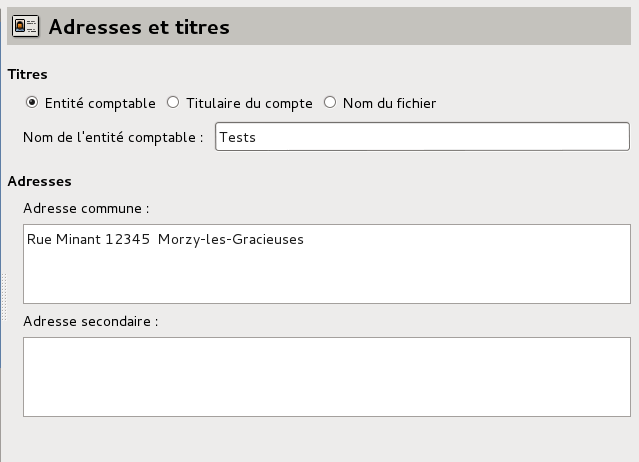
\includegraphics[scale=0.5]{image/screenshot/setup_adresses}
\end{center}
\caption{Adresses et titres}
\label{setup-adresses-img}
\end{figure}
% image centrée 
\fi


\subparagraph{Titre de la fenêtre de Grisbi :\label{setup-display-addresses-titles}}

Grisbi affiche en haut de sa page d'accueil, à droite de l'icône \menu{Grisbi}, un \indexword{titre}\index{affichage !titre}\index{titre !affichage} qui permet d'identifier sur quel document vous travaillez actuellement, sous la forme \og libellé - Grisbi\fg{}. Vous pouvez définir ici ce libellé, parmi les trois suivants :

\begin{itemize}
	\item \menu{Entité comptable} : c'est le nom du domaine de comptabilité sur lequel vous travaillez, par exemple \og Ma comptabilité \fg{} ou \og Association \fg{}, et que vous avez saisi à la création du fichier de comptes ; vous pouvez le modifier ici dans le champ \menu{Nom de l'entité comptable} ; cela peut être utile si vous gérez plusieurs \indexword{entités comptables}\index{entité comptable} ;
	\item \menu{Titulaire du compte} : Grisbi affiche le nom du titulaire (ou du propriétaire) du dernier compte consulté ; si ce titulaire n'est pas renseigné dans les propriétés du compte, Grisbi affiche le nom de ce compte ;
	\item \menu{Nom du fichier} : c'est le \indexword{nom du fichier}\index{fichier de comptes !nom}\index{nom !fichier de comptes} dans le répertoire courant, sous la forme \file{nom\_de\_\_votre\_fichier.gsb}, et c'est le choix par défaut.
\end{itemize}


\subparagraph{Adresses :\label{setup-display-addresses-address}}

Vous pouvez indiquer ici deux adresses différentes (commune et secondaire), dans les deux champs juste en-dessous.


\subsection{Tiers, catégories et imputations budgétaires\label{setup-display-third}}

Cet onglet permet de définir certains paramètres d'affichage de ces trois \ifIllustration onglets\refimage{setup-thirdCategories-img}.
% image centrée
\begin{figure}[h!]
\begin{center}
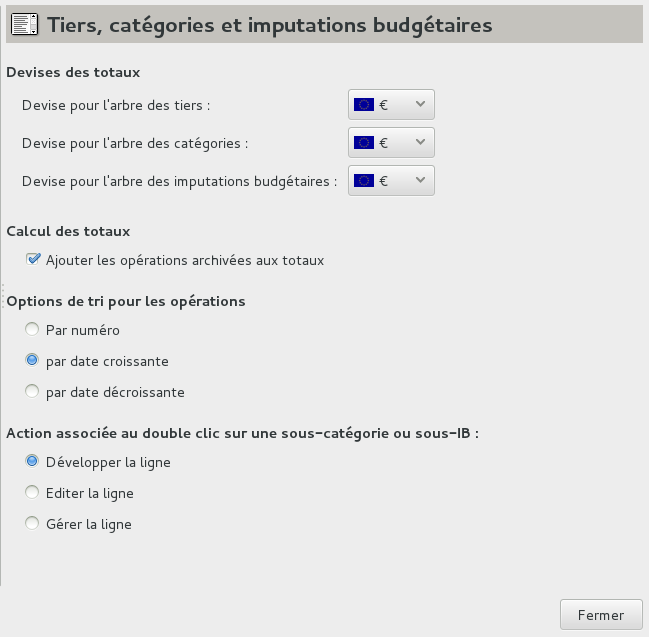
\includegraphics[scale=0.5]{image/screenshot/setup_thirdCategories}
\end{center}
\caption{Tiers, catégories et imputations budgétaires}
\label{setup-thirdCategories-img}
\end{figure}
% image centrée
\else onglets.
\fi


\subparagraph{Devises des totaux :\label{setup-display-third-currencies}}

Vous pouvez ici définir individuellement la \indexword{devise utilisée pour les totaux}\index{devise !totaux} des différents onglets \menu{Tiers}, \menu{Catégories} et \menu{Imputations budgétaires} du panneau de navigation. Pour chacun, sélectionnez la devise dans la liste déroulante correspondante. Le choix ne peut être fait que parmi les devises que connaît votre fichier de comptes (voir la section \vref{setup-resources-currencies}, \menu{Devises}).


\subparagraph{Calcul des totaux :\label{setup-display-third-sum}}

La case \menu{Ajouter les opérations archivées aux totaux}, cochée par défaut, permet de tenir ou non compte des opérations archivées dans le \indexword{calcul des totaux}\index{affichage !totaux}\index{calcul des totaux !affichage}, pour les onglets \menu{Tiers}, \menu{Catégories} et \menu{Imputations budgétaires}. Lorsque cette option est cochée, les totaux dans ces onglets comptabilisent les opérations archivées. Dans le cas contraire les totaux ne comptabilisent que les opérations non archivées.

% espace avant Attention ou Note  : 5 mm
\vspacepdf{5mm}
\strong{Attention} : ne décochez cette case qu'en connaissance de cause, car ces totaux risqueraient alors de ne pas refléter la réalité !


\subparagraph{Action associée au double clic sur une sous-catégorie ou sous-IB :\label{setup-display-third-mouse}}

Vous pouvez définir l'action qu'exécutera le \indexword{double-clic} de la souris\index{sous-catégories !double-clic}\index{sous-imputations budgétaires !double-clic} sur une sous-catégorie ou une sous-imputation budgétaire, parmi les choix suivants :
\begin{itemize}
	\item Développer la ligne : c'est le choix par défaut ;
	\item Éditer la ligne ;
	\item Gérer la ligne.
\end{itemize}

\subparagraph{Option pour les associations françaises :\label{setup-display-third-french}}

La case \menu{Remplacer Revenus/Dépenses par Produits/Charges} devrait être cochée pour les associations qui utilisent le Plan Comptable Général français, car Produits et Charges sont les dénominations officielles. 


\subparagraph{Option de tri pour les opérations :\label{setup-display-third-sort}}

Vous pouvez choisir l'\indexword{ordre d'affichage des opérations}\index{tri !opérations}, parmi trois critères de \gls{tri} :

\begin{itemize}
	\item tri par numéro : c'est le choix par défaut ;
	\item tri par date croissante ;
	\item tri par date décroissante.
\end{itemize} 


\subparagraph{Afficher une liste courte d'entrées dans la zone de sélection des tiers :\label{setup-display-third-list}}

Vous pouvez cocher ou non la case \menu{Limiter le nombre de tiers dans la zone de sélection des tiers}. Cela permet de limiter la liste de tiers à ceux utilisés par les opérations non archivées VÉRIFIER SI LA CORRECTION SERA FAITE PAR PIERRE (MESSAGE DU 10/03/21 19:12). 

En effet, lorsque vous cherchez un tiers dans le formulaire de saisie des opérations (voir la section \vref{transactions-new}, \menu{Saisie d'une nouvelle opération}), vous entrez les premières lettres de ce tiers, et une liste déroulante apparaît qui vous propose tous les tiers commençant par ces lettres ; la liste peut être très longue et la recherche du tiers peut être tout aussi longue ; cette option permet de réduire la taille de la liste déroulante, en particulier en ignorant les tiers correspondant à des opérations archivées, donc à priori anciennes. 
Si vous cochez la case, une fenêtre s'ouvre et vous donne une explication sur le bon choix à faire, mais vous pouvez choisir ce que vous voulez.


\subsection{Éléments de l'interface\label{setup-display-toolbars}}

Plusieurs éléments de l'interface utilisateur de Grisbi peuvent être configurés. Il s'agit :

\begin{itemize}
	\item de la résolution de l'écran ;
	\item de la barre d'information ;
	\item du panneau de navigation ;
	\item des barres d'outils ;
	\item des raccourcis clavier.
\end{itemize}

Pour identifier correctement les trois premiers, voir le chapitre \vref{home}, \menu{Accueil} \ifIllustration \refimage{setup-toolbar-img}.
% image centrée
\begin{figure}[htbp]
\begin{center}
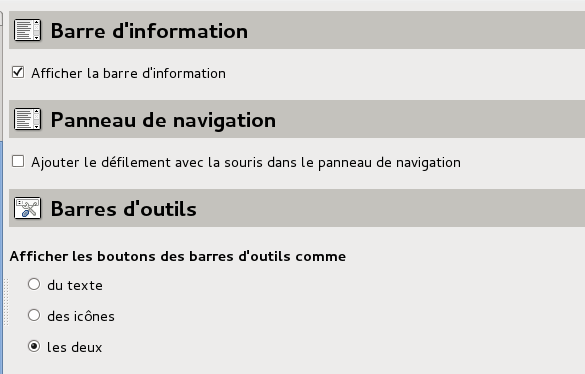
\includegraphics[scale=0.5]{image/screenshot/setup_toolbar}
\end{center}
\caption{Éléments de l'interface}
\label{setup-toolbar-img}
\end{figure}
% image centrée
\else .
\fi

\subparagraph{Résolution de l'écran :}

Cette fonction permet d'améliorer l'utilisation de Grisbi si l'on utilise un écran de faible résolution. Une fois modifiée, la prise en compte se fait en fermant la fenêtre des préférences puis en la réouvrant.



\subparagraph{Barre d'information :}

La barre d'information\index{barre d'information !affichage} (voir la section \vref{home-synthesis}) peut être affichée ou non en (dé)cochant la case correspondante \menu{Afficher la barre d'information}. .

\subparagraph{Panneau de navigation :}

Dans ce panneau \index{panneau de navigation !défilement} (voir la section \vref{home-accounting}), vous pouvez choisir la possibilité de faire défiler les onglets avec la molette de la souris, en cochant la case \menu{Ajouter le défilement avec la souris dans le panneau de navigation} : c'est le choix par défaut. Dans ce cas, l'onglet qui défile est l'onglet précédemment sélectionné, en rose foncé{\couleur}.


\subparagraph{Barre d'outils :}

Vous pouvez choisir le mode d'affichage des boutons de la barre d'outils\index{barre d'outils !boutons}(voir la section \vref{transactions-functions}), avec :
\begin{itemize}
	\item du \menu{Texte seul} ;
	\item des \menu{Icônes seules} ;
	\item du \menu{Texte sous  les icônes}, c'est le choix par défaut ;
	\item du \menu{Texte à côté des icônes}.
\end{itemize}




\subparagraph{Raccourcis clavier :}

La liste des raccourcis clavier utilise ici les libellés « Alt » et « Primary » : si la touche Alt est nommée ainsi sur tous les claviers, d'autres modificateurs ont des libellés différents en fonction du clavier ou du système ; voici les correspondances les plus courantes :

\begin{itemize}
	\item pour Windows et Linux, Primary = touche CTRL ;
	\item pour Mac, Primary = touche Commande ou Cmd.
\end{itemize}



\section{Opérations\label{setup-operations}}


\subsection{Comportement de la liste des opérations\label{setup-operations-list}}

Cet onglet permet de configurer la liste \ifIllustration des opérations\refimage{setup-listBehaviour-img}.
% image centrée
\begin{figure}[ht]
\begin{center}
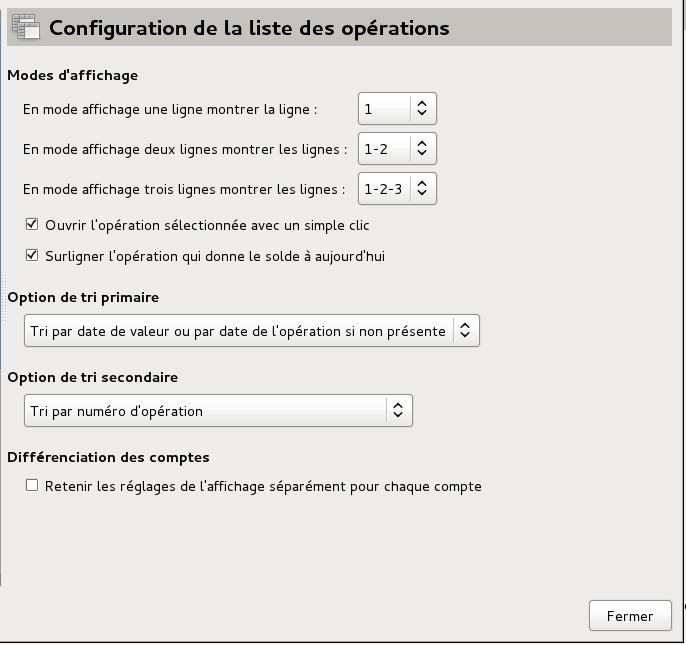
\includegraphics[scale=0.5]{image/screenshot/setup_listBehaviour}
\end{center}
\caption{Configuration de la liste des opérations}
\label{setup-listBehaviour-img}
\end{figure}
% image centrée
\else des opérations.
\fi


\subparagraph{Modes d'affichage :\label{setup-operations-list-modes}}

Dans la liste des opérations, Grisbi vous permet d'afficher de 1 à 4 lignes pour chaque opération (voir la section \vref{transactions-list-description}). 

Vous pouvez choisir le \indexword{mode d'affichage} de la liste des opérations\index{affichage !nombre de lignes}\index{affichage !modes}, c'est à dire l'\indexword{ordre des lignes} qui sont affichées pour toutes les opérations, et cela en fonction du nombre de lignes que vous voudrez afficher : pour les modes d'affichage 2 ou 3 lignes, sélectionnez, dans la liste déroulante  correspondante, l'ordre des lignes affichées. Les modes d'affichage à 1 ou 4 lignes ne peuvent  évidemment être configurés, car ils affichent soit la première ligne, soit toutes les lignes dans l'ordre 1-2-3-4.

VÉRIFIER LES INDEX

\textbf{Note} : le contenu de chaque ligne choisie dépend de la configuration de l'affichage des champs : voir la section \vref{setup-operations-cells}, \menu{Cellules de la liste des opérations}.
% espace après Attention ou Note  : 5 mm
\vspacepdf{5mm}



\subparagraph{Options de la liste des opérations :}

Vous pouvez choisir les fonctions suivantes, à votre convenance :
\begin{itemize}
	\item \menu{Ouvrir l'opération sélectionnée avec un simple clic\index{affichage !opérations}} : c'est le choix par défaut ;
	\item \menu{Surligner l'opération qui donne le solde à aujourd'hui}\index{solde !affichage de l'opération} : le \indexword{surlignage}\index{affichage !surlignage} permet de distinguer l'opération qui donne le solde du jour en coloriant son fond de façon spécifique ; c'est utile lorsque l'on exécute par avance des opérations futures, et c'est le choix par défaut. Cela prend effet quand on a réouvert le compte : l'opération est surlignée en vert{\couleur}.
\end{itemize}


\subparagraph{Option de tri primaire :}

Le \indexword{tri primaire}\index{tri !primaire} sert à déterminer la date pour laquelle le  solde est calculé après chaque opération. Vous pouvez choisir l'un de ces deux critères pour ce tri primaire :

\begin{itemize}
	\item \menu{Tri par date de valeur (par date de l'opération si absente)} : les opérations sont triées par date de valeur ; dans le cas où cette date n'est pas renseignée, elle est remplacée par la date de l'opération ; c'est le \gls{tri} par défaut de Grisbi ;
	\item \menu{Tri par date de valeur puis par date de l'opération} : les opérations sont triées par date de valeur, et pour chaque date, elles sont triées par date de l'opération ;
	\item \menu{Tri forcé par date de l'opération}. 
\end{itemize}

% espace avant Attention ou Note  : 5 mm
\vspacepdf{5mm}
\textbf{Note} : le choix du tri primaire fait ici modifie nécessairement la chronologie des opérations, donc le solde calculé après chaque ligne d'opération.

% espace avant Attention ou Note  : 5 mm
\vspacepdf{5mm}
\textbf{Note} : pour trier les opérations par date d'opération ou par date de valeur, il faut qu'une colonne de la liste des opérations affiche cette date (voir la section \vref{transactions-list-fields}, \menu{Champs d'information et de saisie}), et que vous ayez sélectionné \menu{Date d'opération} ou \menu{Date de valeur} dans le menu contextuel par un clic-droit dans le libellé de la colonne (voir la section \vref{transactions-list-sorts}, \menu{Tris}).


\subparagraph{Option de tri secondaire :}

Vous pouvez choisir l'un de ces quatre critères pour le \indexword{\gls{tri secondaire}}\index{tri !secondaire} :

\begin{itemize}
	\item \menu{Tri par numéro d'opération} : c'est le tri par défaut de Grisbi ;
	\item \menu{Tri par montant (crédit débit)} ;
	\item \menu{Tri par tiers ou par numéro d'opération si non présent} : les opérations sont triées par tiers ; dans le cas où le tiers n'est pas renseigné, le tri est fait par numéro d'opération ;
	\item \menu{Tri par date puis par numéro d'opération} : les opérations sont triées par date, et pour chaque date, elles sont triées par numéro d'opération.
\end{itemize}


\subparagraph{Différenciation des comptes :\label{setup-operations-list-differenciation}}

La \indexword{différenciation des comptes}\index{affichage !comptes}
\index{compte !affichage différencié} est la possibilité de régler leur affichage indépendamment : vous pouvez choisir de \menu{Retenir les réglages de l'affichage séparément pour chaque compte} en cochant la case correspondante.





\subsection{Cellules de la liste des opérations\label{setup-operations-cells}}

Vous pouvez définir le nombre et l'emplacement exact des champs des opérations dans la liste des opérations, grâce aux deux tableaux 
\ifIllustration décrits ci-dessous\refimage{setup-listCells-img}.
\else décrits ci-dessous.
\fi

\ifIllustration
% image centrée
\begin{figure}[ht]
\begin{center}
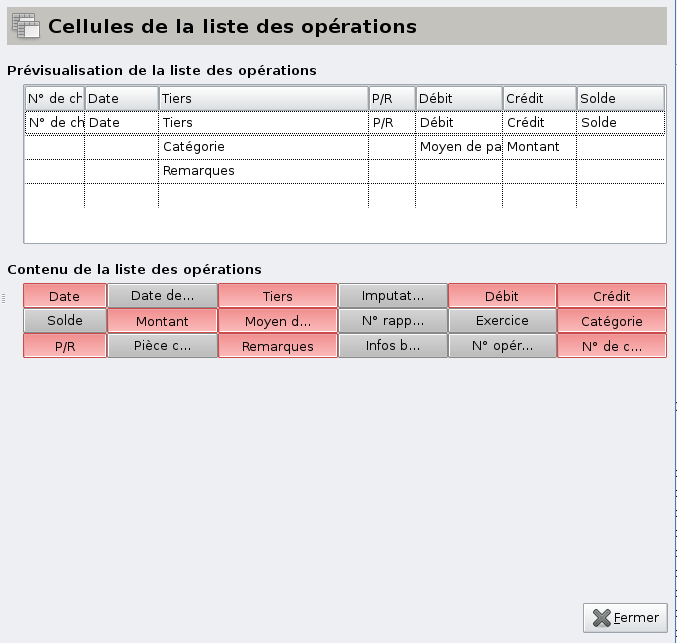
\includegraphics[scale=0.5]{image/screenshot/setup_listCells}
\end{center}
\caption{Cellules de la liste des opérations}
\label{setup-listCells-img}
\end{figure}
% image centrée
\fi

\textbf{Note} : la disposition de l'affichage des champs des opérations dans la liste des opérations des comptes est totalement indépendante de celle de  l'affichage des champs dans le formulaire de saisie, qui est elle-même décrite dans la section \vref{setup-form-content}, \menu{Contenu}.

\ifIllustration
\else
% espace avant Attention ou Note  : 5 mm
\vspacepdf{5mm}
\fi


\subparagraph{Prévisualisation de la liste des opérations :\label{setup-operations-cells-display}}

Le tableau de prévisualisation représente les 7 colonnes et les lignes permettant d'afficher les \indexword{champs d'une opération}\index{champ d'information !aperçu}, qui sont affichés de la même manière, pour chaque opération, dans la liste des opérations de l'onglet \menu{Opérations} de chaque compte.

Ce tableau comprend donc aussi sept colonnes et quatre lignes, qui définissent 28 \indexword{cellules}\index{cellule !définition}, pouvant donc afficher au maximum 28 champs (voir la section \vref{transactions-list-fields}, \menu{Champs d'information et de saisie}.). Vous pouvez modifier la \indexword{largeur des colonnes}\index{colonne !largeur} en cliquant, dans la ligne des libellés des colonnes, sur le séparateur entre deux d'entre-elles (sans relâcher) et en le déplaçant avec la souris.

% espace avant Attention ou Note  : 5 mm
\vspacepdf{5mm}
\textbf{Note} : dans ce tableau, le \indexword{libellé de chaque colonne}\index{colonne !libellé} (en grisé) est toujours celui du champ de la première ligne de cette colonne, quand il est rempli, tout à fait comme dans la liste des opérations.
% espace après Attention ou Note  : 5 mm
\vspacepdf{5mm}

Un même champ ne peut être présent que dans une seule cellule de ce tableau, ainsi que dans la liste des opérations.

% espace pour changement de thème
\vspacepdf{5mm}
Dans ce tableau, vous pouvez \indexword{déplacer un champ}\index{champ d'information !déplacer}
 d'une cellule à une autre cellule en cliquant (sans relâcher) sur son nom et en le déplaçant dans l'autre cellule. Si celle-ci contient déjà un champ, celui-ci disparaît et doit être éventuellement remis en place dans une autre cellule. Il est donc conseillé de ne déplacer un champ que dans une cellule déjà vide.


\subparagraph{Contenu de la liste des opérations :}\index{affichage !lignes d'opérations\label{setup-operations-cells-fields}}

Le tableau montre tous les \indexword{champs affichables}\index{champ !affichable} dans la prévisualisation, donc dans la liste des opérations. Il sert à choisir les champs affichés dans la prévisualisation. Le fond de chaque cellule de ce tableau peut avoir deux couleurs :

\begin{itemize}
	\item gris foncé{\couleur} quand ce champ ne se trouve pas déjà dans la prévisualisation et qu'on peut l'y mettre ;
	\item rouge{\couleur} quand ce champ se trouve déjà dans la prévisualisation.
\end{itemize}

% espace pour changement de thème
\vspacepdf{5mm}
Pour \indexword{ajouter un champ} dans la prévisualisation\index{champ d'information !ajouter}, cliquez sur son nom (sur fond gris foncé{\couleur}) dans le tableau de contenu : la couleur de sa cellule passe au rouge{\couleur}, tandis que le nom de ce champ apparaît dans les dernières lignes du tableau de prévisualisation. Déplacez ensuite ce champ dans la cellule qui vous convient.

% espace pour changement de thème
\vspacepdf{5mm}
Pour \indexword{enlever un champ} de la  prévisualisation\index{champ d'information !enlever}, cliquez sur son nom (sur fond rouge{\couleur}) dans le tableau de contenu : la couleur de sa cellule passe au gris foncé{\couleur}, tandis que ce champ disparaît de la prévisualisation.

\ifIllustration
% espace pour changement de thème
\vspacepdf{5mm}
\fi

% espace pour changement de thème
\vspacepdf{5mm}

Pour \indexword{modifier un champ} de la  prévisualisation\index{champ d'information !modifier}, déplacez-le dans une autre cellule et ajoutez un autre champ à la place.

\textbf{Note} : il est possible d'enlever tous les champs du tableau de prévisualisation, et dans ce cas la liste des opérations ne contiendra l'\indexword{affichage d'aucune opération} \index{affichage !aucune opération}.

% espace pour changement de thème
\vspacepdf{5mm}
Grisbi vous offre une très grande \indexword{souplesse} pour l'affichage des \indexword{champs des opérations}\index{affichage !champ des opérations}\index{affichage !souplesse} dans la liste des opérations des comptes : d'une part, vous pouvez positionner n'importe quel champ d'information sur n'importe quelle cellule de n'importe laquelle des quatre lignes du tableau de prévisualisation ; d'autre part, le menu \menu{Mode d'affichage} de la liste d'opérations permet quatre possibilités d'affichage (\menu{Vue simple}, \menu{Mode \og deux lignes \fg{}}, \menu{Mode \og trois lignes \fg{}} et \menu{Vue complète}), qui peuvent être configurés dans le paragraphe \vref{setup-operations-list-modes}, \menu{Modes d'affichage}. Vous pouvez donc, suivant le \menu{Mode d'affichage} sélectionné, afficher quatre jeux de lignes que vous voulez, par exemple :

\begin{itemize}
	\item \menu{Vue simple} : affichage de la ligne 1 ;
	\item \menu{Mode \og deux lignes \fg{}} : affichage des lignes 3-4 ;
	\item \menu{Mode \og trois lignes \fg{}} : affichage des lignes 1-2-4 ;
	\item \menu{Vue complète} : affichage des lignes 1-2-3-4, évidemment.
\end{itemize}

ou toute autre combinaison.


\subsection{Messages avant suppression\label{setup-operations-remove}}

\subparagraph{Afficher les messages de suppression suivants :}

En (dé)cochant la case correspondante, vous pouvez autoriser ou non l'affichage des messages suivants :

\begin{itemize}
	\ifIllustration
	% image entourée par une liste (picins)
	% pas de référence à l'illustration car erreur de numéro de figure avec picins.
	% supprimé car en html les figures entourées ne sont pas numérotées, et la numérotation des figures centrées décalée par rapport au pdf
	%\piccaption{Messages avant suppression}
	\label{setup-messagesDelete-img}
	\parpic[r]{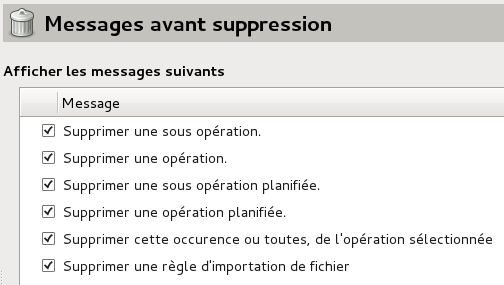
\includegraphics[scale=0.5]{image/screenshot/setup_messagesDelete}}
	% image entourée par une liste
	\fi
	\item \menu{Supprimer une sous-opération} ;
	\item \menu{Supprimer une opération} ;
	\item \menu{Supprimer une sous-opération planifiée} ;
	\item \menu{Supprimer une opération planifiée} ;
	\item \menu{Supprimer une ou toutes les occurrences de l'opération sélectionnée} ; 
	\item \menu{Supprimer une règle d'importation de fichier}.
\end{itemize}

\ifIllustration
% espace après légende  : 10 mm
\vspacepdf{20mm}
\fi

Par défaut, l'affichage de tous ces messages est validé.

\ifIllustration
% espace après image entourée
\vspacehevea{13mm}
\fi


\subsection{Rapprochement\label{setup-operations-reconciliation}}

Cet onglet permet de gérer \ifIllustration les rapprochements effectués antérieurement \refimage{setup-reconciliation-img}. 

% image centrée
\begin{figure}[htb]
\begin{center}
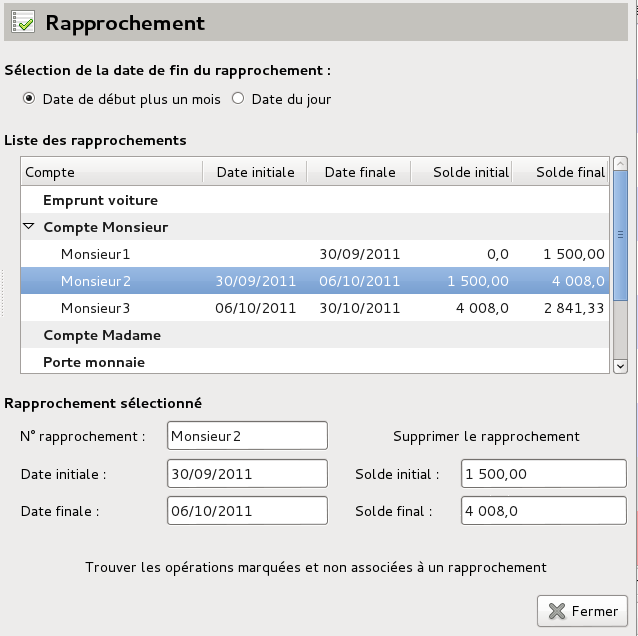
\includegraphics[scale=0.5]{image/screenshot/setup_reconciliation}
\end{center}
\caption{Gestion des rapprochements antérieurs}
\label{setup-reconciliation-img}
\end{figure}
% image centrée
\else les rapprochements effectués antérieurement.
\fi

Voir le chapitre \vref{reconciliation}, \menu{Rapprochement bancaire}. 


\subparagraph{Sélection de la date de fin de rapprochement :\label{setup-operations-reconciliation-date}}

Vous pouvez définir la date de fin de rapprochement\index{rapprochement !date de fin}
 parmi ces deux dates :
\begin{itemize}
	\item \menu{Date de début plus un mois} ; c'est la date par défaut ;
	\item \menu{Date du jour}.
\end{itemize}


\subparagraph{Liste des rapprochements :}\index{rapprochements !liste\label{setup-operations-reconciliation-list}}

Le tableau \indexword{liste tous les rapprochements}\index{rapprochement !liste} déjà effectués dans tous les comptes de votre fichier de comptes. 

Pour afficher tous les rapprochements d'un ou plusieurs comptes, cliquez sur le petit triangle à gauche de leurs noms. Vous pouvez alors sélectionner un des rapprochements par un clic sur sa ligne, son numéro s'affiche dans la colonne \menu{Compte}, et ses dates (initiale et finale) et soldes (initial et final) s'affichent dans leurs colonnes respectives.

\textbf{Note} : ces petits triangles peuvent être remplacés, en fonction du thème de l'environnement de bureau ou du gestionnaire de fenêtres que vous utilisez, par d'autres caractères tels que +, -, >, <, etc.

% espace pour changement de thème
\vspacepdf{5mm}

La case \menu{Tri des rapprochements par date décroissante} permet de trouver plus facilement certains rapprochements. 

À sa droite, le bouton \menu{Regrouper la ligne}  permet de réenrouler le contenu des rapprochements d'un compte qui a été auparavant déroulé par son petit triangle noir à sa gauche. Ce bouton permet de réenrouler plus rapidement plusieurs comptes.


\subparagraph{Rapprochement sélectionné :}\index{rapprochement !caractéristiques\label{setup-operations-reconciliation-selection}}

Quand vous sélectionnez un rapprochement dans le tableau, le détail de ses caractéristiques apparaît dans les différents champs en-dessous, que vous pouvez modifier en cas de besoin.

% espace pour changement de thème
\vspacepdf{5mm}
Le bouton \menu{Supprimer le rapprochement}\index{rapprochement !supprimer} permet de \indexword{supprimer le rapprochement} sélectionné ; dans ce cas, toutes les opérations rapprochées liées à ce rapprochement perdront leur statut d'opérations rapprochées, retrouveront le statut d'opérations pointées et seront donc marquées \og \textbf{P} \fg{} dans la liste des opérations. 

% espace avant Attention ou Note  : 5 mm
\vspacepdf{5mm}
\strong{Attention} : la suppression d'un rapprochement, la modification ou la suppression de certaines caractéristiques d'un rapprochement, peuvent avoir des conséquences importantes sur le compte concerné, par exemple sur la cohérence entre les dates (initiale et finale), ou entre les soldes (initial et final) de deux rapprochements consécutifs, pouvant aller jusqu'à rendre votre fichier de comptes inutilisable. Il est donc fortement conseillé de faire une \textbf{copie de sauvegarde} de votre fichier de comptes auparavant.

% espace après Attention ou Note  : 5 mm
\vspacepdf{5mm}

Le bouton \menu{Trouver les opérations marquées et non associées à un rapprochement}\index{rapprochement !opérations non associées} permet d'aider à rétablir une continuité des rapprochements et de réparer certaines erreurs. Les \indexword{opérations marquées}\index{opération !marquée} correspondent à des opérations qui peuvent avoir une lettre \og \textbf{P} \fg{}, \og \textbf{R} \fg{} ou \og \textbf{T} \fg{} dans la colonne \menu{P/R} de la liste des opérations. Si vous cliquez sur ce bouton, l'assistant \menu{Associer des opérations orphelines à un rapprochement}s'ouvre, qui permet de  :

\begin{itemize}
	\item créer directement à la main autant de rapprochements que nécessaire, juste par leur date et soldes ;
	\item associer automatiquement les opérations orphelines à un rapprochement existant et correspondant à sa date ; cela est très pratique pour les opérations orphelines créées par l'usage incorrect de la touche \key{Ctrl}\key{R} ;
	\item associer manuellement les opérations orphelines à des rapprochements existants.
\end{itemize}


\subsection{Options de tri pour les rapprochements\label{setup-operations-sort}}

\subparagraph{Rapprochement : tri des opérations :}

Vous pouvez configurer ici l'ordre d'affichage des opérations, dans la liste des opérations\index{rapprochement !tri des opérations}, lors d'un rapprochement des opérations d'un compte (voir le chapitre \vref{reconciliation}, \menu{Rapprochement bancaire}). Cet ordre peut être configuré par un \gls{tri} selon les modes de règlement. Cela peut être utile si votre relevé bancaire présente un ordre particulier selon ces modes de règlement, et si vous voulez faire correspondre l'affichage de Grisbi avec \ifIllustration ce relevé\refimage{setup-reconciliation-sort-img}.
% image centrée
\begin{figure}[htbp]
\begin{center}
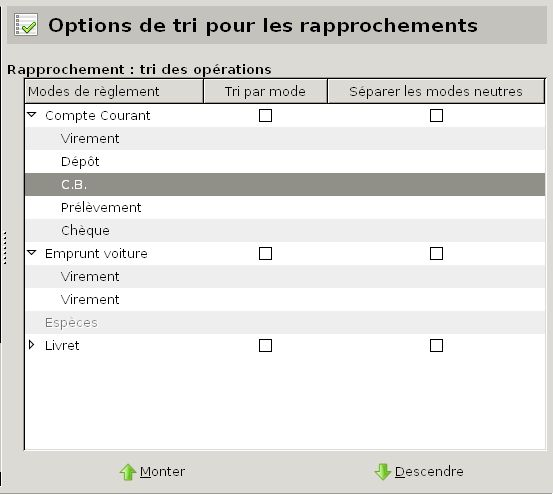
\includegraphics[scale=0.5]{image/screenshot/setup_reconciliation_sort}
\end{center}
\caption{Options de tri pour les rapprochements}
\label{setup-reconciliation-sort-img}
\end{figure}
% image centrée
\else ce relevé.
\fi

Un tableau affiche la liste des comptes de votre fichier de comptes. Pour afficher tous les modes de règlement d'un ou plusieurs comptes, cliquez sur le petit triangle à gauche de leur nom.

\textbf{Note} : ces triangles peuvent être remplacés, en fonction du thème de l'environnement de bureau ou du gestionnaire de fenêtres que vous utilisez, par d'autres caractères tels que +, -, >, <, etc.

%espace après Attention ou Note : 5 mm
\vspacepdf{5mm}
Vous pouvez choisir, individuellement pour chaque compte, que les opérations de votre compte se présentent triées par mode de règlement.

Vous pouvez aussi, individuellement pour chaque compte, y \menu{Séparer les modes neutres}\index{rapprochement !mode neutre} : un \indexword{mode neutre} est un mode de règlement qui peut être indifféremment un débit ou un crédit, comme par exemple un virement, au contraire du mode \menu{Prélèvement} qui est toujours un débit, ou du mode  \menu{Dépôt} qui est toujours un crédit. 

% espace pour changement de thème
\vspacepdf{5mm}
Pour ajuster un ordre particulier pour un compte, procédez comme suit :
\begin{enumerate}
	\item cliquez sur le petit triangle à gauche du nom du compte concerné, pour en dérouler le contenu ;
	\item cliquez, sur la ligne du compte concerné, dans la case de la colonne \menu{Tri par mode} ;
	\item cliquez, sur la même ligne, dans la case de la colonne \menu{Séparer les modes neutres}, si vous le voulez : ces modes s'ordonnent du positif en haut au négatif en bas ;
	\item cliquez sur l'un des modes de règlement et déplacez-le à la position voulue avec les boutons \menu{Monter} ou \menu{Descendre} ; **********************CES ACTIONS NE FONCTIONNENT PAS ****************************** RAPPORT DE BOGUE EST FAIT
	\item recommencez cette action sur les autres modes jusqu'à l'obtention de l'ordre de \gls{tri} voulu pour ce compte.
\end{enumerate}

% espace pour changement de thème
\vspacepdf{5mm}

Le bouton \menu{Tout Regrouper} permet de réenrouler tous les affichages des modes de tous les comptes.


\section{Formulaire des opérations\label{setup-form}}


\subsection{Comportement du formulaire\label{setup-form-behaviour}}

\subparagraph{Appuyer sur ENTRÉE dans le formulaire de saisie des opérations :\label{setup-form-behaviour-enter}}
 


\ifIllustration
% image centrée
\begin{figure}[htbp]
	\begin{center}
		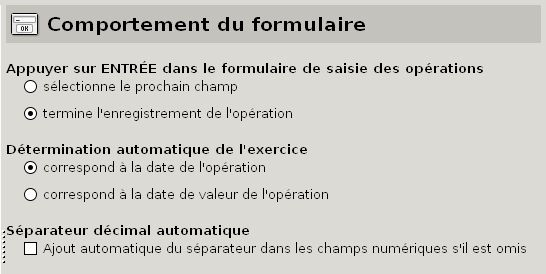
\includegraphics[scale=0.5]{image/screenshot/setup_formBehaviour}
	\end{center}
	\caption{Comportement du formulaire des opérations}
	\label{setup-formBehaviour-img}
\end{figure}
% image centrée
\fi

L'appui sur la \indexword{touche \key{Entrée}}\index{formulaire de saisie !touche \key{Entrée}} peut déclencher l'une ou l'autre des fonctions suivantes :

\begin{itemize}
	\item \menu{sélectionne le prochain champ} ; c'est le choix par défaut ;
	\item \menu{termine l'enregistrement de l'opération}.
\end{itemize}


%\ifIllustration formulaire\refimage{setup-formBehaviour-img} :
%\else formulaire :
%\fi


\subparagraph{Interprétation des dates futures :\label{setup-form-behaviour-future}}

Une opération future est une opération dont la date est postérieure à la date courante ; quand vous entrez une opération future dans le formulaire de saisie de la liste des opérations, et non dans l'échéancier, et si  cochez la case \menu{Remplacer l'année des dates futures par l'année précédente}, l'année de cette opération est remplacée par l'année précédente. Cela permet de ne pas risquer de perdre de vue cette opération.

\subparagraph{Détermination automatique de l'exercice :\label{setup-form-behaviour-financialyear}}

La \indexword{Détermination automatique de l'exercice}\index{formulaire de saisie !détermination de l'exercice} se fait de l'une ou l'autre des manières suivantes :

\begin{itemize}
	\item \menu{correspond à la date de l'opération} : c'est le choix par défaut ;
	\item \menu{correspond à la date de valeur de l'opération}.
\end{itemize}



\subparagraph{Trier les exercices en descendant dans la boîte de saisie du formulaire :\label{setup-form-behaviour-sort}}

Lorsque vous entrez les premiers chiffres d'un exercice, une liste déroulante vous permet de choisir directement l'exercice voulu ; vous pouvez trier les exercices dans l'ordre descendant ou montant, en cochant ou non la case \menu{Trier les exercices en descendant}.
	
\subparagraph{Séparateur décimal automatique :\label{setup-form-behaviour-decimal}}

Vous pouvez cocher ou non la case \menu{Ajout automatique du séparateur dans les champs numériques s'il est omis} : le \indexword{séparateur décimal} \index{formulaire de saisie !séparateur décimal}peut devenir automatique, ou non, de cette manière.


\subparagraph{Sélection de l'opération après validation de l'opération ventilée :\label{setup-form-behaviour-selection}}

Quand vous avez terminé la dernière sous-opération d'une opération ventilée METTRE DANS L'INDEX, vous pouvez valider l'ensemble, et cette validation aura pour effet, au choix, de :

\begin{itemize}
	\item \menu{Sélectionner une nouvelle opération} : c'est le choix par défaut ;
	\item \menu{Sélectionner l'opération ventilée}.
\end{itemize}




\subsection{Contenu\label{setup-form-content}}

Vous pouvez définir le nombre et l'emplacement exact des champs constituant le formulaire de saisie des opérations, grâce aux deux tableaux \ifIllustration décrits ci-dessous\refimage{setup-transactions-form-img}.
% image centrée
\begin{figure}[htbp]
\begin{center}
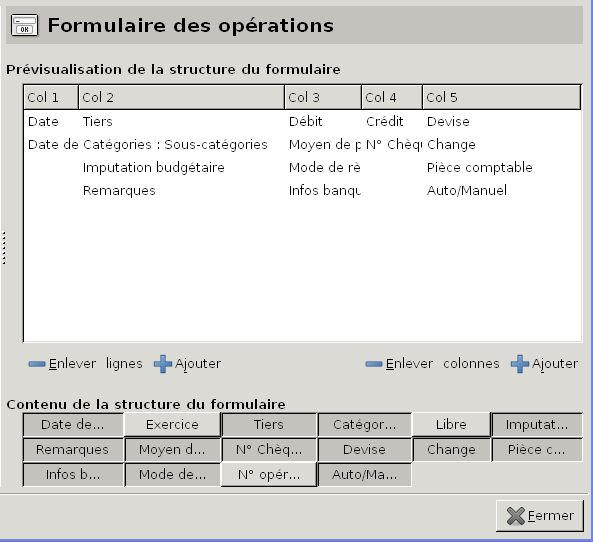
\includegraphics[scale=0.5]{image/screenshot/setup_transactions_form}
\end{center}
\caption{Formulaire des opérations}
\label{setup-transactions-form-img}
\end{figure}
% image centrée
\else décrits ci-dessous.
\fi

\textbf{Note} : la disposition de l'affichage des champs dans le formulaire de saisie est totalement indépendante de celle de  l'affichage des champs dans la liste des opérations des comptes, qui est elle-même décrite dans la section \vref{setup-operations-cells}, \menu{Cellules de la liste des opérations}.


\subparagraph{Prévisualisation de la structure du formulaire :\label{setup-form-content-display}}

Ce tableau présente un aperçu des champs du formulaire de saisie des opérations tels qu'ils sont affichés dans l'onglet \menu{Opérations} d'un compte.

Le formulaire peut avoir de 1 à 4 lignes et de 4 à 6 colonnes. Vous pouvez en diminuer ou augmenter le nombre grâce aux boutons \menu{Enlever} et \menu{Ajouter} à côté des libellés \menu{lignes} et \menu{colonnes}, sous ce tableau à gauche et à droite. Vous pouvez modifier la \indexword{largeur des colonnes}\index{colonne !largeur} en cliquant sur le séparateur entre deux d'entre-elles (sans relâcher) et en le déplaçant avec la souris.

% espace avant Attention ou Note  : 5 mm
\vspacepdf{5mm}
\textbf{Note} : bien que les colonnes de ce tableau soient nommées ici \og Col 1 \fg{} à \og Col 6 \fg{}, le libellé d'une colonne dans le formulaire de saisie (dans la liste des opérations d'un compte) est \emph{toujours} le libellé du champ situé sur la première ligne de ce tableau de prévisualisation.
% espace après Attention ou Note  : 5 mm
\vspacepdf{5mm}
 
Une \indexword{cellule}\index{cellule !définition} est définie par l'intersection d'une ligne et d'une colonne. Un champ donné ne peut être présent que dans une seule cellule du formulaire.


\subparagraph{Contenu de la structure du formulaire :\label{setup-form-content-fields}}

Ce tableau montre tous les champs affichables dans le tableau de prévisualisation. Il sert à positionner les champs affichés dans la prévisualisation. Chaque cellule de ce tableau peut avoir deux couleurs :

\begin{itemize}
	\item gris clair quand ce champ ne se trouve pas déjà dans la prévisualisation et qu'on peut l'y mettre ;
	\item gris foncé quand ce champ se trouve déjà dans la prévisualisation.
\end{itemize}

Les champs \menu{Date}, \menu{Débit} et \menu{Crédit} ne sont pas mentionnés, car ils sont obligatoires et figurent déjà dans le tableau de prévisualisation.

% espace pour changement de thème
\vspacepdf{5mm}
Pour \indexword{déplacer un champ}\index{champ de saisie !déplacer} d'une cellule à une autre cellule, cliquez (sans relâcher) sur son nom et déplacez-le dans l'autre cellule. Si celle-ci n'est pas vide, les deux champs sont intervertis.

% espace pour changement de thème
\vspacepdf{5mm}
Pour \indexword{ajouter un champ} dans la prévisualisation\index{champ de saisie !ajouter}, cliquez sur son nom dans le tableau de contenu : la couleur de sa cellule passe au gris foncé, tandis que le nom de ce champ apparaît dans la prévisualisation. La première ligne se complète d'abord si elle a des cellules vides, sinon la suivante fait de même, etc.

% espace pour changement de thème
\vspacepdf{5mm}

Pour \indexword{enlever un champ} de la  prévisualisation\index{champ de saisie !enlever}, cliquez sur son nom dans le tableau de contenu : la couleur de sa cellule passe au gris clair, tandis que ce champ disparaît de la prévisualisation.

% espace avant Attention ou Note  : 5 mm
\vspacepdf{5mm}
\textbf{Note} : il est impossible d'enlever les champs  \menu{Date}, \menu{Débit} et \menu{Crédit}, car ce sont les informations minimales indispensables à une opération.

% espace avant Attention ou Note  : 5 mm
\vspacepdf{5mm}
\textbf{Note} : les champs \menu{Devise} et \menu{Change} sont liés dans le tableau de contenu : la configuration de l'affichage du champ \menu{Devise} dans la prévisualisation y positionne automatiquement le champ \menu{Change}, et inversement ; vous pouvez ensuite les déplacer dans les cellules voulues.


\subsection{Aide à la saisie du formulaire\label{setup-form-help}}


\subparagraph{Options communes :\label{setup-form-help-common}}

Vous pouvez ou non cocher la case \menu{Remplissage sensible à la casse METTRE DANS L'INDEX ET LE GLOSSAIRE} \indexword{casse}\index{caractères !casse} des caractères ;

Vous pouvez définir le \menu{Nombre minimum de caractères avant proposition dans les champs de saisie} avec les boutons \menu{+} et \menu{-} : lorsque dans un champ du formulaire de saisie vous entrez les premiers caractères d'un mot ou d'un nombre, Grisbi vous affiche une liste déroulante pour vous aider à le compléter ; cette liste apparaît quand ce nombre minimum de caractères est dépassé.

\subparagraph{Options pour les tiers :\label{setup-form-help-third}}

En cochant la case \menu{Remplissage automatique des opérations à partir du tiers}, vous validez la possibilité des choix suivants :

\begin{itemize}
	\item \menu{Effacer le champ \menu{Crédit} ou \menu{Débit}} ;
	\item \menu{Récupérer automatiquement les sous-opérations de l'opération associée} : les champs des sous-opérations sont remplis avec les données de la dernière opération ventilée ayant le même tiers que celui déjà saisi ;
	\item \menu{Limiter le remplissage avec des tiers appartenant au compte courant} : la recherche de l'opération se fait dans le compte courant ; si la case n'est pas cochée, elle se fait dans la totalité des comptes.
\end{itemize}

% espace pour changement de thème
\vspacepdf{5mm}

%\ifIllustration fonctions suivantes\refimage{setup-enterHelp-img} :
%\else fonctions suivantes :
%\fi

Vous pouvez aussi \menu{Ne pas permettre la création de nouveau tiers} en cochant sa case.

% espace pour changement de thème
\vspacepdf{5mm}

\subparagraph{Options pour les catégories et imputations budgétaires :\label{setup-form-categories}}

Vous pouvez choisir les options :

\begin{itemize}

	\item \menu{Mélanger les catégories de débit/crédit} : lorsque l'on déroule la liste des catégories, elles sont triées par ordre alphabétique plutôt que par débit puis crédit ;
	\item \menu{Ne pas permettre la création de nouvelles catégories/imputations budgétaires}.
\end{itemize}

\ifIllustration
% image centrée
\begin{figure}[ht]
\begin{center}
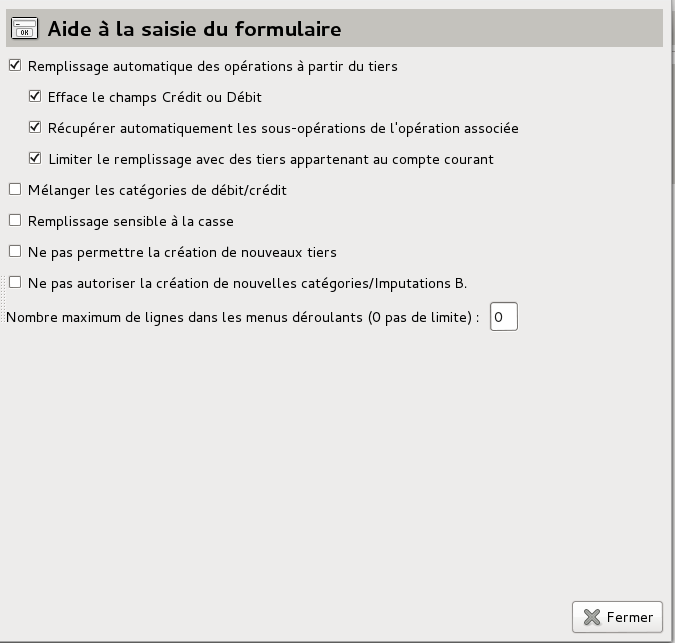
\includegraphics[scale=0.5]{image/screenshot/setup_enterHelp}
\end{center}
\caption{Aide à la saisie du formulaire}
\label{setup-enterHelp-img}
\end{figure}
% image centrée
\fi




\section{Ressources\label{setup-resources}}


\subsection{Devises\label{setup-resources-currencies}}

Cet onglet affiche le tableau des \indexword{devises connues}\index{devise !connue} par votre fichier de comptes, ainsi que les \indexword{propriétés de la devise}\index{devise !propriétés} \ifIllustration sélectionnée \refimage{setup-currencies-img}. 
\else sélectionnée.
\fi

\subparagraph{Devises connues :\label{setup-resources-currencies-known}}

Le tableau affiche les noms des pays et les \indexword{devises connues}\index{devise !connue} par votre fichier de comptes, ainsi que ses nom, code ISO et symbole monétaire.

% espace pour changement de thème
\vspacepdf{5mm}

Juste en-dessous deux boutons \menu{Ajouter} et \menu{Enlever} permettent de gérer ce tableau.


% \indexword{propriétés de la devise}\index{devise !propriétés} \ifIllustration sélectionnée \refimage{setup-currencies-img}. 
%\else sélectionnée.

\ifIllustration
% image centrée
\begin{figure}[ht]
\begin{center}
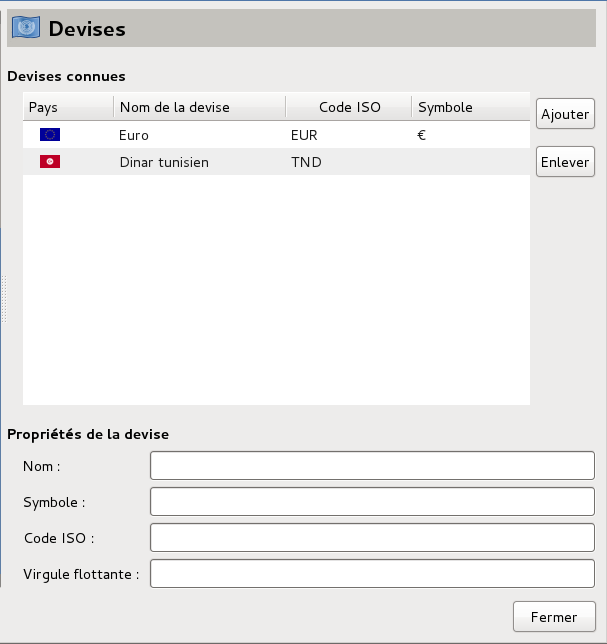
\includegraphics[scale=0.5]{image/screenshot/setup_currencies}
\end{center}
\caption{Configuration des devises}
\label{setup-currencies-img}
\end{figure}
% image centrée
\fi

%Cette fonction n'est plus présente pour les devises de l'euro, mais devrait être possible pour les futures candidates à l'euro :
%Vous pouvez aussi indiquer si les devises passeront à l'euro lorsque vous choisirez de basculer la tenue d'un compte dans cette monnaie (ceci est probablement obsolète pour beaucoup d'utilisateurs, mais certains peuvent en avoir encore besoin).


% espace pour changement de thème
\vspacepdf{5mm}

\subparagraph{Propriétés de la devise :\label{setup-resources-currencies-properties}}

Si vous cliquez sur la ligne d'une devise dans le tableau des \indexword{devises connues}\index{devise !connue}, les \indexword{propriétés de la devise}\index{devise !propriétés} s'affichent dans cette section.

ATTENTION AU TEXTE LIÉ À L'IMAGE

% \ifIllustration sélectionnée \refimage{setup-currencies-img}. 
%\else sélectionnée.
%\fi

Les différents champs permettent de \indexword{configurer la devise}\index{devise !configurer} sélectionnée : Nom, Symbole monétaire, Code ISO, ainsi que le nombre de chiffres après la virgule. Le symbole monétaire est généralement disponible sur votre clavier ; par exemple, vous pouvez saisir \key{AltGr}\key{e} pour le symbole de l'Euro.


\ifIllustration
\else
% espace pour changement de thème
\vspacepdf{5mm}
\fi
Pour \indexword{ajouter une devise}\index{devise !ajouter}, procédez comme suit :

\begin{enumerate}
	\item cliquez sur le bouton \menu{Ajouter} : la fenêtre de sélection de la devise s'affiche ;
	\item cherchez le pays ou la devise dans la liste ; si vous ne trouvez pas, cochez la case \menu{Afficher les devises obsolètes} pour afficher d'\indexword{anciennes devises}\index{devise !ancienne} ;
	\item cliquez dans la liste sur la ligne du pays ou de la devise choisie ;
	\item  si besoin, modifiez les propriétés de la devise dans la section \menu{Propriétés de la devise} ;
	\item validez par le bouton \menu{Ajouter} : la devise s'affiche dans le tableau \menu{Devises connues}.
\end{enumerate}

% espace pour changement de thème
\vspacepdf{5mm}
Pour \indexword{modifier une devise}\index{devise !modifier}, sélectionnez-la dans le tableau \menu{Devises connues} et modifiez-la dans la section \menu{Propriétés de la devise}.

% espace pour changement de thème
\vspacepdf{5mm}
Pour \indexword{supprimer une devise}\index{devise !supprimer}, sélectionnez-la dans le tableau \menu{Devises connues} et cliquez sur le bouton \menu{Enlever}.

% espace avant Attention ou Note  : 5 mm
\vspacepdf{5mm}
\textbf{Note} : si vous essayez de supprimer une devise utilisée dans une opération d'un de vos comptes, Grisbi affichera une fenêtre de refus.


%Section «Liens entre devises»  : tout  le texte et le début de «Banques» se trouvent dans la marge de bas de page et sont illisibles quand le tableau des devises de la zone euro est présent. Donc Tableau et texte de présentation  SUPPRIMÉS
%
%Pour information, le tableau ci-dessous reprend les taux de conversion en euro des monnaies de la zone euro. Depuis le 1 \ier janvier 1999, ces taux sont fixés de manière définitive et irrévocable. Le tableau exprime la valeur de 1 euro dans chaque monnaie. Cette valeur se compose d'une séquence de six chiffres significatifs (par ex. : 1 EUR = xx,xxxx BEF). 
%\begin{longtable}{|l|c|r|}
%\hline 
%Devise          & Abréviation & Taux\\
%\hline
%\hline 
%Franc belge          & BEF & 40,3400\\
%\hline 
%Schilling autrichien & ATS & 13,7603\\
%\hline 
%Mark allemand        & DEM & 1,95583\\
%\hline*
%Peseta espagnole     & ESP & 166,386\\
%\hline 
%Mark finlandais      & FIM & 5,94573\\
%\hline 
%Franc français       & FRF & 6,55957\\
%\hline 
%Livre irlandaise     & IEP & 0,78756\\
%\hline 
%Lire italienne       & ITL & 1936,27\\
%\hline 
%Franc luxembourgeois & LUF & 40,3399\\
%\hline 
%Florin néerlandais   & NLG & 2,20371\\
%\hline 
%Escudo portugais     & PTE & 200,482\\
%\hline 
%Drachme grecque      & GRD & 340,750\\
%\hline
%\end{longtable}
%
%Section «Liens entre devises»  : tout  le texte et le début de «Banques» se trouvent dans la marge de bas de page et sont illisibles quand le tableau des devises de la section euro est présent. Donc Tableau et texte de présentation  SUPPRIMÉS


\subsection{Liens entre devises\label{setup-resources-rate}}

Cet onglet affiche le tableau des \indexword{liens existants}\index{devise !liens existants} créés dans votre fichier de comptes, ainsi que les \indexword{propriétés du lien}\index{devise !propriétés} \ifIllustration sélectionné. \refimage{setup-currencies-img}. 
\else sélectionnée.
\fi





%% image centrée 
%\begin{figure}[htbp]
%\begin{center}
%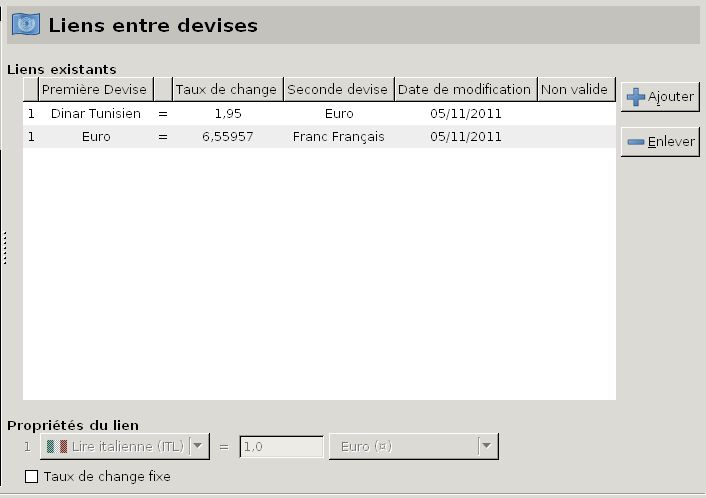
\includegraphics[scale=0.5]{image/screenshot/setup_exchangerate}
%\end{center}
%\caption{Configuration des taux de change}
%\label{setup-exchangerate-img}
%\end{figure}
%% image centrée 
%\else détails.
%\fi

\subparagraph{Liens existants :\label{setup-resources-rate-existing}}

Le tableau affiche les liens précédemment établis entre deux devises, donc les taux de change, sous la forme « 1 Euro = 6,55957 Franc », avec la dernière date de modification de ce taux de change.

Juste en-dessous deux boutons \menu{Ajouter} et \menu{Enlever} permettent de gérer ce tableau.




 %votre fichier de comptes, ainsi que les \indexword{propriétés du lien}\index{lien !propriétés} \ifIllustration sélectionnée ; il %permet aussi de \indexword{gérer les taux de change}\index{taux de change !gérer}, \ifIllustration %détails\refimage{setup-exchangerate-img}.


\subparagraph{Propriétés du lien :\label{setup-resources-rate-properties}}

Si vous cliquez sur la ligne d'un lien dans le tableau des \indexword{liens existants}\index{devise !liens existants}, les \indexword{propriétés du lien}\index{devise !liens existant} s'affichent dans cette section.

Cette ligne contient les données du lien, sous la forme « 1 Euro = 6,55957 Franc », avec la dernière date de modification de ce taux de change. C'est ici que vous pouvez modifier le taux de change.



%espace pour changement de thème
\vspacepdf{5mm}
Pour \indexword{ajouter un lien entre deux devises}\index{lien entre devises !ajouter}, procédez comme suit :

\begin{enumerate}
	\item cliquez sur le bouton \menu{Ajouter} : une nouvelle ligne de lien s'affiche dans le tableau \menu{Liens existants}  ;
	\item sélectionnez ce lien par un clic sur sa ligne ;
	\item dans la section  \menu{Propriétés du lien}, définissez la devise de départ et celle d'arrivée grâce aux deux listes déroulantes, et saisissez le taux de change dans le champ entre ces deux listes ; faites attention à respecter la formule « Devise 1 = Taux de change Devise 2 ;
	  % espace pour notte alignée avec l'item
	  
	  \textbf{Note} : vous pouvez inverser le sens de la conversion (Devise 1 =  Taux de change Devise 2, ou bien Devise2 = Taux de change Devise 1) en inversant le nom des devises dans les deux listes déroulantes ; vous pouvez ainsi entrer exactement le taux de change tel qu'il vous est communiqué. 
	\item cochez la case \menu{Taux de change fixe} si c'est le cas ;
	\item validez par le bouton \menu{Fermer}.
\end{enumerate}

%espace pour changement de thème
\vspacepdf{5mm}
Pour \indexword{modifier un lien entre deux devises}\index{lien entre devises !modifier}, sélectionnez-le dans le tableau \menu{Liens existants} et modifiez le taux de change dans la section \menu{Propriétés du lien}.

%espace pour changement de thème
\vspacepdf{5mm}
Pour \indexword{supprimer un lien entre deux devises}\index{lien entre devises !supprimer}, sélectionnez-le sélectionnez-le dans le tableau \menu{Liens existants} et cliquez sur le bouton \menu{Enlever}.

% espace avant Attention ou Note  : 5 mm
\vspacepdf{5mm}
\textbf{Note} : si vous essayez de supprimer un lien d'une devise utilisée dans une opération d'un de vos comptes, Grisbi affichera une fenêtre de refus.


\subsection{Banques\label{setup-resources-banks}}

Cet onglet affiche le tableau des \indexword{banques connues}\index{banques !liste} dans votre fichier de comptes, ainsi que les \indexword{détails de la banque}\index{banque !détails} \ifIllustration sélectionnée \refimage{setup-bank-img}. 
\else sélectionnée.
\fi




VOIR IMAGE
%Cet onglet \indexword{liste les banques}\index{banques !liste} connues par votre fichier de comptes, ainsi que
%\ifIllustration tous leurs détails\refimage{setup-bank-img}.
%\else tous leurs détails.
%\fi



\ifIllustration
% image centrée
\begin{figure}[ht!]
\begin{center}
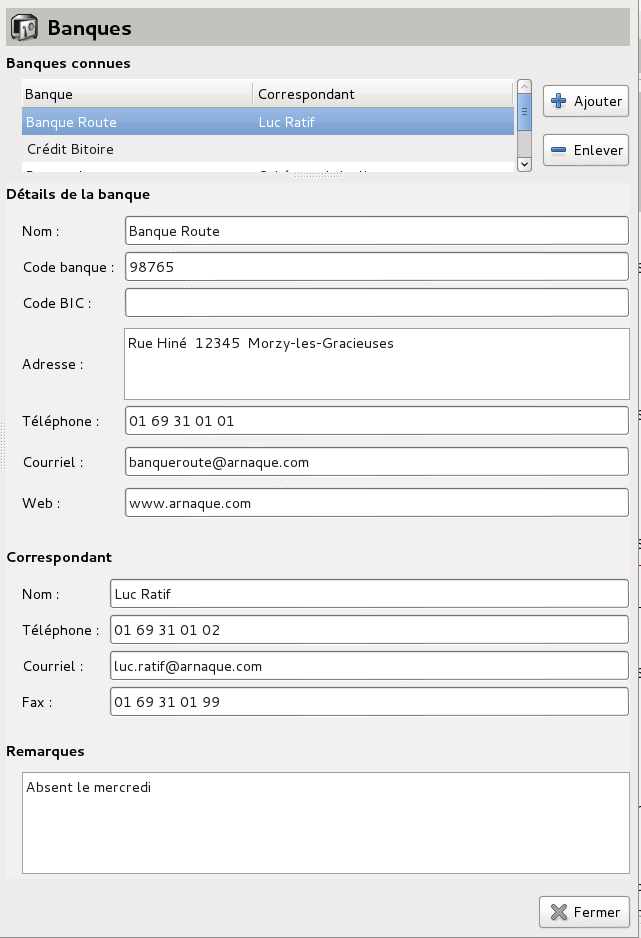
\includegraphics[scale=0.48]{image/screenshot/setup_bank}
\end{center}
\caption{Configuration des établissements financiers}
\label{setup-bank-img}
\end{figure}
% image centrée
\fi


\subparagraph{Banques connues :\label{setup-resources-banks-known}}


Le tableau affiche la liste de ces banques, avec le nom du contact que vous avez avec chacune, si vous l'avez renseigné auparavant. 


Juste en-dessous deux boutons \menu{Ajouter} et \menu{Enlever} permettent de gérer ce tableau.

 


\subparagraph{Détails de la banque :\label{setup-resources-banks-details}}

%Si vous sélectionnez une banque par un clic sur la ligne d'une banque dans le tableau des \menu{Banques connues} , les \menu{Détails de la banque} affichent, groupés sous trois rubriques \menu{Généralités}, \menu{Correspondant} et \menu{Remarques} tous les \indexword{détails sur la banque}\index{banque !détails} que vous avez entrés auparavant dans Grisbi. 


Si vous cliquez sur la ligne d'une banque dans le tableau des \indexword{banques connues}\index{banque !connues}, tous les \indexword{détails de la banque}\index{banque !détails} que vous avez entrés auparavant dans Grisbi s'affichent dans cette section, groupés sous trois rubriques \menu{Généralités}, \menu{Correspondant} et \menu{Remarques}.




% espace pour changement de thème
\vspacepdf{5mm}


% espace pour changement de thème
\vspacepdf{5mm}
Pour \indexword{ajouter une banque}\index{banque !ajouter}, procédez comme suit :

\begin{enumerate}
	\item cliquez sur le bouton \menu{Ajouter} : une nouvelle ligne \menu{Nouvelle banque} s'affiche dans le tableau \menu{Banques connues} ;
	\item sélectionnez cette banque par un clic sur sa ligne ;
	\item dans la section \menu{Détails de la banque}, saisissez ses nom, code, Code BIC, et toutes autres informations utiles dans les nombreux champs prévus ;
	\item validez par le bouton \menu{Fermer}.
\end{enumerate}

\ifIllustration
\else
% espace pour changement de thème
\vspacepdf{5mm}
\fi

Pour \indexword{modifier une banque}\index{banque !modifier}, sélectionnez-la dans le tableau \menu{Banques connues} et modifiez-en ses détails.

% espace pour changement de thème
\vspacepdf{5mm}
Pour \indexword{supprimer une banque}\index{banque !supprimer}, sélectionnez-la dans le tableau \menu{Banques connues}, cliquez sur le bouton \menu{Enlever}, puis validez dans la fenêtre de confirmation.

% espace avant Attention ou Note  : 5 mm
\vspacepdf{5mm}
\strong{Attention} : la suppression d'une banque est irréversible.




\subsection{Exercices\label{setup-resources-financialyear}}

Cet onglet affiche le tableau des \indexword{exercices définis}\index{exercice !défini} dans votre fichier de comptes, ainsi que les \indexword{détails sur l'exercice}\index{exercice !détails} \ifIllustration sélectionné \refimage{setup-currencies-img}. 
\else sélectionné.
\fi



%permet de créer de nouveaux exercices, et de modifier ou supprimer des exercices \ifIllustration existants\refimage{setup-financialyear-img}.
%\else existants.
%\fi







\ifIllustration
% image centrée
\begin{figure}[ht]
\begin{center}
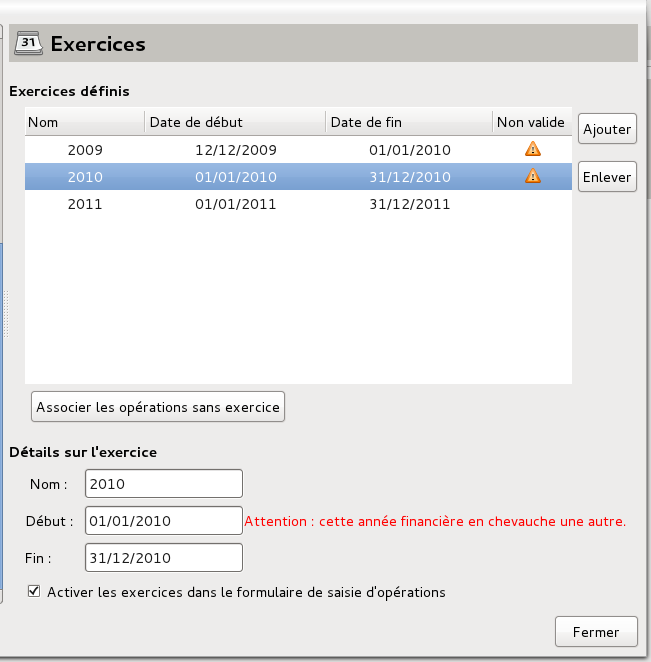
\includegraphics[scale=0.5]{image/screenshot/setup_financialyear}
\end{center}
\caption{Configuration des exercices}
\label{setup-financialyear-img}
\end{figure}
% image centrée
\fi

% espace pour changement de thème
\vspacepdf{5mm}

\subparagraph{Exercices définis :\label{setup-resources-financialyear-list}}

Le tableau affiche la \indexword{liste des exercices}\index{exercice !liste} déjà définis dans votre fichier de comptes.

% espace pour changement de thème
\vspacepdf{5mm}
Vous pouvez cocher ou non la case \menu{Trier les exercices en mode descendant}.



% espace pour changement de thème
\vspacepdf{5mm}
Juste en-dessous deux boutons \menu{Ajouter} et \menu{Enlever} permettent de gérer ce tableau, et le bouton \menu{Associer les opérations sans exercice} permet d'attribuer automatiquement aux opérations l'exercice correspondant à la date de l'opération.

% espace pour changement de thème
\vspacepdf{5mm}



\subparagraph{Détails sur l'exercice :\label{setup-resources-financialyear-details}}

%Si vous sélectionnez un exercice par un clic sur la ligne d'un exercice dans le tableau des \menu{Banques connues} , les \menu{Détails de la banque} affichent, groupés sous trois rubriques \menu{Généralités}, \menu{Correspondant} et \menu{Remarques} tous les \indexword{détails sur la banque}\index{banque !détails} que vous avez entrés auparavant dans Grisbi.


Si vous cliquez sur la ligne d'un exercice dans le tableau des \indexword{exercices définis}\index{exercices !définis}, tous les \indexword{détails sur l'exercice}\index{exercices !détails} que vous avez entrés auparavant dans Grisbi s'affichent dans la section \menu{Détails sur l'exercice}.

% espace pour changement de thème
\vspacepdf{5mm}




% espace pour changement de thème
\vspacepdf{5mm}
Pour \indexword{ajouter un exercice}\index{exercice !ajouter}, procédez comme suit :

\begin{enumerate}
	\item cliquez sur le bouton \menu{Ajouter} : une nouvelle ligne \menu{Nouvel exercice} s'affiche dans la section \menu{Détails sur l'exercice} ;
	\item saisissez-y son nom et ses dates de début et de fin : les dates peuvent être saisies, comme dans le formulaire de saisie des opérations, au clavier (voir la section \vref{transactions-new-dates}, \menu{Saisie de date au clavier}) ou au calendrier (voir la section \vref{transactions-new-calendar}, \menu{Saisie de date au calendrier}) ;
	\item cliquez sur le bouton \menu{Associer les opérations sans exercice}, si vous voulez que votre nouvel exercice soit affecté automatiquement à toutes les opérations correspondantes ; si vous validez la fenêtre qui s'affiche ensuite, Grisbi affiche le nombre d'opérations qui ont été associées à l'exercice concerné ;
	\item cochez la case \menu{Activer les exercices dans le formulaire de saisie d'opérations}, si vous voulez afficher un champ  \menu{Exercice} dans le formulaire de saisie, et ainsi pouvoir entrer un exercice lors de la saisie des opérations ;
	\item validez par le bouton \menu{Fermer}.
\end{enumerate}

\textbf{Note} : les exercices ne doivent pas se chevaucher ; si c'est le cas, Grisbi affiche un message d'alerte en rouge{\couleur} \ifIllustration \refimage{setup-financialyear-img}.
\else .
\fi

% espace pour changement de thème
\vspacepdf{5mm}
Pour \indexword{modifier un exercice}\index{exercice !modifier}, sélectionnez-le dans la section \menu{Détails sur l'exercice} et modifiez-en ses détails.

%% espace pour changement de thème
\vspacepdf{5mm}
Pour \indexword{supprimer un exercice}\index{exercice !supprimer}, sélectionnez-le dans la section \menu{Détails sur l'exercice}, cliquez sur le bouton \menu{Enlever}, puis validez la fenêtre de confirmation. 

% espace avant Attention ou Note  : 5 mm
\vspacepdf{5mm}
\textbf{Note} : cette suppression ne fait que supprimer l'exercice sélectionné dans le tableau \menu{Exercices définis}, ainsi que le champ \menu{Exercice} dans le formulaire de saisie des opérations et dans toutes les opérations qui y sont associées. Mais en aucun cas elle ne supprime les opérations elles-mêmes\ldots

% espace pour changement de thème
\vspacepdf{5mm}
Le bouton \menu{Associer les opérations sans exercice}\index{exercice !opérations sans exercice}\index{opération !sans exercice} permet d'attribuer automatiquement un exercice à toutes les opérations qui en sont dépourvues, en fonction de leur date d'opération (ou de leur date de valeur). C'est aussi le bouton \emph{magique} dans le cas d'un fichier importé d'une ancienne version (ou au format QIF) ; si vous validez la fenêtre qui s'affiche ensuite, Grisbi affiche le nombre d'opérations qui ont été associées à l'exercice concerné.


À VÉRIFIER AVEC PIERRE

%Fonctionnement à vérifier ultérieurement
La case \menu{Activer les exercices dans le formulaire de saisie d'opérations}\index{formulaire de saisie !activer un exercice}\index{exercice !activer} permet d'\indexword{activer l'affichage des exercices} dans ce formulaire, à l'endroit où vous l'aurez défini dans la section PRÉFÉRENCES FORMULAIRE DES  OPÉRATIONS À DÉFINIR XXXXXXXXXXX et ainsi d'entrer un exercice lors de la saisie des opérations. Si cela n'est pas le cas, vous devrez le faire manuellement dans le menu \menu{Édition - Préférences} (voir la section \vref{setup-form-content}, \menu{Contenu} et éventuellement la section \vref{transactions-list-fields}, \menu{Champs d'information et de saisie}).
%Fonctionnement à vérifier ultérieurement. L'affichage devrait être automatique dans le formulaire et dans la liste des opérations
Vous pouvez aussi désactiver l'affichage des exercices en décochant la case \menu{Activez les exercices dans le formulaire de saisie d'opérations}.
S'il est désactivé, et si vous rappelez, dans le formulaire de saisie des opérations, une opération dont l'exercice n'est plus affiché, la mention \menu{Automatique} apparaîtra à la place du libellé de l'exercice.

À VÉRIFIER AVEC PIERRE

\subsection{Modes de règlement\label{setup-resources-modes}}


Cet onglet affiche le tableau des \indexword{modes de règlement}\index{mode de règlement !liste} disponibles dans votre fichier de comptes, ainsi que les \indexword{Détails du mode de règlement}\index{mode de règlement !détails}
\ifIllustration sélectionné \refimage{setup-currencies-img}. 
\else sélectionné.


%qui apparaissant dans la liste déroulante\index{mode de règlement !liste}\index{mode de règlement !détails} du formulaire
%\ifIllustration de saisie des opérations\refimage{setup-modes-img}.
%\else de saisie des opérations.
%\fi 




\fi



\ifIllustration
% image centrée
\begin{figure}[ht]
\begin{center}
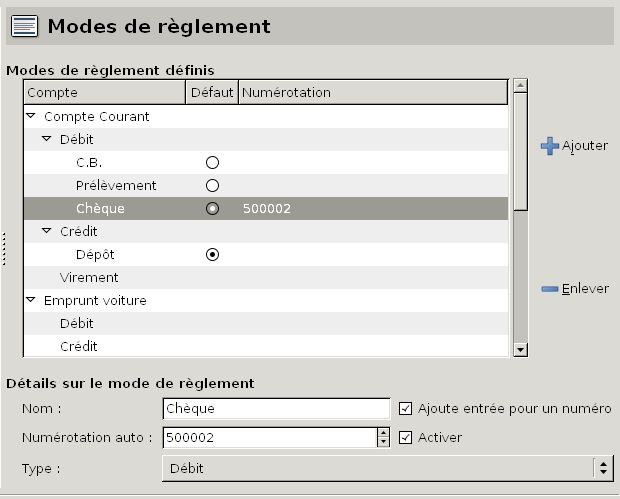
\includegraphics[scale=0.5]{image/screenshot/setup_modes}
\end{center}
\caption{Configuration des modes de règlement}
\label{setup-modes-img}
\end{figure}
% image centrée
\fi

\subparagraph{Modes de règlement :\label{setup-resources-modes-list}}




Le tableau affiche la liste de tous vos comptes dans l'ordre où ils sont affichés dans le panneau de navigation (et non celui où ils ont été créés), précédés d'un petit triangle. Un clic sur ce triangle déroule ou enroule la liste des modes de règlement disponibles pour le compte concerné.

\textbf{Note} : ces triangles peuvent être remplacés, en fonction du thème de l'environnement de bureau ou du gestionnaire de fenêtres que vous utilisez, par d'autres caractères tels que +, -, >, <, etc.

Juste en-dessous trois boutons \menu{Ajouter}, \menu{Enlever} et  \menu{Tout regrouper} permettent de gérer ce tableau.

% espace pour changement de thème
\vspacepdf{5mm}




Ces modes de règlement sont les suivants : 

\begin{itemize}
	\item \menu{Débit} ;
	\item \menu{Crédit} ;
	\item \menu{Virement} : un virement peut être entrant ou sortant. Ce mode doit donc être proposé tant au débit qu'au crédit. Grisbi considère par défaut qu'il est neutre (un mode neutre est un mode de règlement qui peut être indifféremment un débit ou un crédit).
\end{itemize}

Ces modes de règlement dépendent du type de compte : compte de caisse, bancaire, de passif, etc.(voir la sectionXXXXXXXXXX) ; par exemple, un compte de caisse n'a pas le virement comme mode de règlement.

% espace pour changement de thème
\vspacepdf{5mm}
De même, un autre clic sur le triangle devant le type \menu{Débit} déroule ou enroule la liste des modes de règlement disponibles :

\begin{itemize}
	\item \menu{Carte de crédit} ;
	\item \menu{Prélèvement} ;
	\item \menu{Chèque}.
\end{itemize}

Pour le type \menu{Crédit}, le seul mode de règlement disponible est \menu{Dépôt}.

\ifIllustration
\else
% espace pour changement de thème
\vspacepdf{5mm}
\fi




\subparagraph{Détails du  mode de règlement :\label{setup-resources-modes-details}}


Si vous cliquez sur une ligne d'un mode de règlement dans le tableau des \indexword{modes de règlement}\index{mode de règlement !détails}, tous les \indexword{détails du mode de règlement}\index{mode de règlement !détails} que vous avez entrés auparavant dans Grisbi s'affichent dans cette section : Nom, Numérotation automatique et Type.

% espace pour changement de thème
\vspacepdf{5mm}

Pour \indexword{ajouter un nouveau mode de règlement}\index{mode de règlement !ajouter}, procédez comme suit :

\begin{enumerate}
	\item Sélectionnez le compte concerné, ou un de ses deux types \menu{Débit} ou  \menu{Crédit}, par un clic. Le bouton \menu{Ajouter} devient actif ;
	\item cliquez sur le bouton \menu{Ajouter} : une nouvelle ligne \menu{Nouveau mode de règlement} s'affiche, provisoirement dans la section \menu{Débit} ;
	\item sélectionnez ce \menu{Nouveau mode de règlement} par un clic sur sa ligne ;
	\item si vous cliquez sur le bouton dans la colonne  \menu{Défaut}, la liste des modes de paiement sera positionnée par défaut sur ce nouveau mode à chaque nouvelle opération dans ce compte ;
	\item dans la section \menu{Détails sur le mode de règlement} :
		\begin{enumerate}
			\item saisissez son nom dans le champ \menu{Nom} : choisissez un nom pas trop long, pour son affichage correct dans le formulaire de saisie,
			\item si vous cochez la case \menu{Ajouter un numéro}, le champ \menu{\No chèque/virement} est ajouté dans le formulaire de Grisbi pour le mode de règlement sélectionné, et cela valide la case \menu{Activer},
			\item si vous cochez la case \menu{Activer}, l'incrémentation automatique du champ \menu{\No chèque/virement} du formulaire de saisie des opérations est validée ; cette numérotation automatique fonctionne aussi pour tous les modes, c'est à vous d'imaginer ce que vous pouvez en faire (par exemple, vous pouvez numéroter automatiquement vos remises de chèques),
			\item dans le champ \menu{Numérotation auto}, entrez des caractères, dont le dernier devra être numérique, à partir duquel la numérotation commencera, par exemple «Règlement1»,
			\item dans la liste déroulante de libellé  \menu{Type}, choisissez le type d'opération : \menu{Débit}, \menu{Crédit} ou \menu{Neutre} pour un type indifférent.
		\end{enumerate}
\end{enumerate}

\ifIllustration
\else
% espace pour changement de thème
\vspacepdf{5mm}
\fi

Pour \indexword{modifier un mode de règlement}\index{mode de règlement !modifier}, sélectionnez-le dans le tableau \menu{Mode de règlement} et modifiez-en les détails.

% espace pour changement de thème
\vspacepdf{5mm}
Pour \indexword{supprimer un mode de règlement}\index{mode de règlement !supprimer}, sélectionnez-le dans le tableau \menu{Mode de règlement} , cliquez sur le bouton \menu{Enlever}, puis validez dans la fenêtre de confirmation.



\section{Budget prévisionnel\label{setup-budget}}


Cet onglet permet de configurer les différents paramètres des budgets prévisionnels pour les différents comptes de votre fichier de comptes.


\subsection{Généralités\label{setup-budget-general}}

Cet onglet permet de définir les \indexword{paramètres généraux}\index{prévision !paramètres généraux} pour l'ensemble de vos \ifIllustration  budgets\refimage{setup-budgetGeneral-img}.
\else budgets. 
\fi

\ifIllustration
% image centrée
\begin{figure}[h!]
\begin{center}
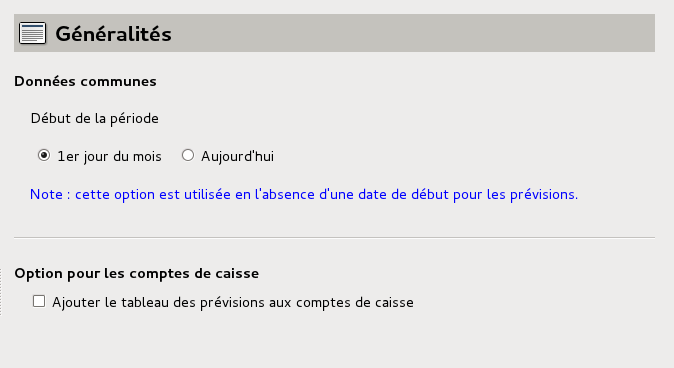
\includegraphics[scale=0.5]{image/screenshot/setup_budget_general}
\end{center}
\caption{Configuration générale des budgets prévisionnels}
\label{setup-budgetGeneral-img}
% image centrée
\end{figure}
\fi

\subparagraph{Données communes :\label{setup-budget-general-common}}

Vous pouvez choisir le \menu{Début de la période} servant de référence pour établir les prévisions, en cliquant sur l'un des deux boutons : soit le \menu{1\up{er} jour du mois} (c'est le choix par défaut), soit \menu{aujourd'hui}. 

\textbf{Note} : cette option est utilisée en l'absence d'une date de début renseignée dans l'onglet \menu{Prévisions} du compte concerné (voir la section \vref{budget-estimate-summary}, \menu{En-tête des prévisions}).
% espace après Attention ou Note  : 5 mm
\vspacepdf{5mm}

\subparagraph{Option pour les comptes de caisse :\label{setup-budget-general-cash}}

Vous pouvez aussi choisir si les \indexword{comptes de caisse}\index{prévision !comptes de caisse} pourront aussi avoir leur tableau de \indexword{prévisions}, en cochant la case \menu{Ajouter le tableau des prévisions aux comptes de caisse}.



\subsection{Données des comptes\label{setup-budget-data}}

Cet onglet permet de valider la fonctionnalité de budget prévisionnel et d'en configurer les paramètres, indépendamment pour chacun des comptes à budgétiser. 

\ifIllustration
% image centrée
\begin{figure}[htbp]
\begin{center}
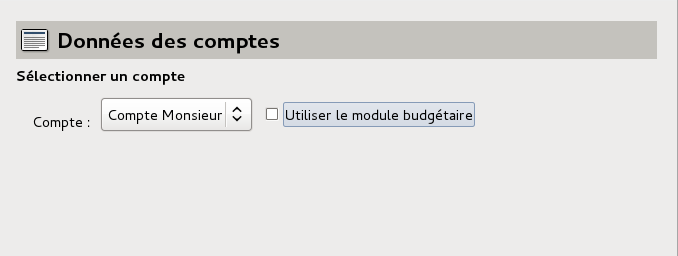
\includegraphics[scale=0.5]{image/screenshot/setup_budget_data1}
\end{center}
\caption{Configuration des budgets : choix des comptes}
\label{setup-budgetData1-img}
\end{figure}
% image centrée
\fi

\subparagraph{Sélectionnez un compte :\label{setup-budget-data-select}}

La section \menu{Sélectionnez un compte} \ifIllustration affiche\refimage{setup-budgetData1-img} :
\else affiche : 
\fi

\begin{itemize}
	\item une liste déroulante pour choisir le compte sur lequel vous voulez faire les prévisions ;
	\item la case à cocher \menu{Utiliser le module budgétaire}, pour \indexword{valider le module budgétaire}\index{module budgétaire !valider} pour ce compte ; 
	
%	si vous la cochez, une case à cocher \menu{Compte avec carte à débit différé} apparaît juste en-dessous, et une nouvelle section intitulée \menu{Données...} s'affiche dessous, dans laquelle vous pourrez configurer le module budgétaire ; les données de cette section seront fonction du type de compte que vous aurez choisi.
\end{itemize}


% espace pour changement de thème
\vspacepdf{5mm}
%Plusieurs comptes peuvent ainsi faire l'objet de prévisions, indépendamment et simultanément. 

% espace pour changement de thème
\vspacepdf{5mm}
Pour \indexword{configurer le module budgétaire}\index{module budgétaire !configurer} pour un compte, sélectionnez ce compte dans la liste déroulante, puis cochez la case \menu{Utiliser le module budgétaire}. 

Une autre case à cocher de libellé \menu{Compte avec carte à débit différé} apparaît juste en-dessous, et une nouvelle section intitulée \menu{Données...} s'affiche dessous, dans laquelle vous pourrez configurer le module budgétaire ; les données de cette section seront différentes en fonction du type de compte que vous aurez choisi :


\begin{itemize}
	\item type compte de passif ;
	\item type compte bancaire ;
	\item type compte de caisse ;		
	\item type compte de passif avec carte bancaire à débit différé ;	
	\item type compte bancaire avec carte bancaire à débit différé ;
	\item type compte de caisse avec carte bancaire à débit différé ;
	\item type compte d'actif.	
\end{itemize}		


\subparagraph{Données du crédit pour Type compte de passif :\label{setup-budget-data-liability}}

Pour les comptes de passif, une case à cocher et une seule section supplémentaire \ifIllustration s'affichent\refimage{setup_budget_dataLiability-img} :
\else s'affichent :
\fi

\begin{itemize}
	\item la case de libellé \menu{Compte avec carte à débit différé} ; 
	\item la section \menu{Données du crédit}.
\end{itemize}

\ifIllustration
% image centrée
\begin{figure}[ht]
\begin{center}
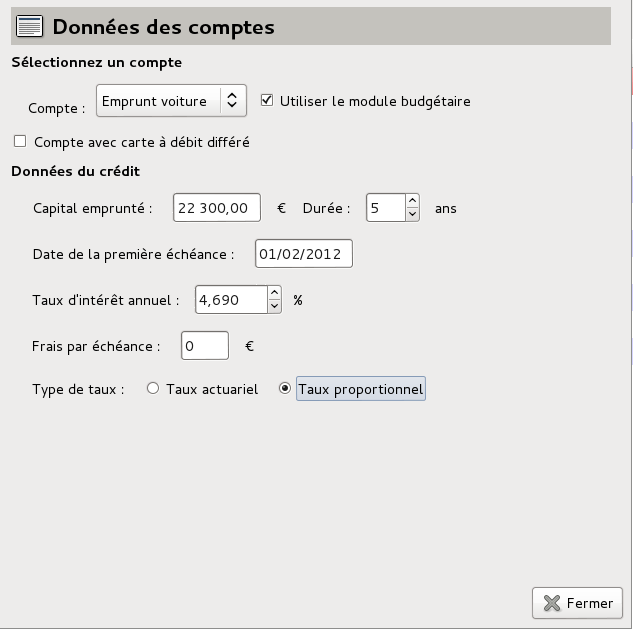
\includegraphics[scale=0.5]{image/screenshot/setup_budget_dataLiability}
\end{center}
\caption{Configuration d'un budget pour un compte de passif}
\label{setup_budget_dataLiability-img}
\end{figure}
% image centrée
\fi

De plus, dans le pavé des détails du compte concerné (voir la section     ), un nouvel onglet \menu{Tableau d'amortissement} s'est ajouté entre les deux autres onglets \menu{Opérations} et \menu{Propriétés}.

% espace pour changement de thème
\vspacepdf{5mm}
Pour configurer les prévisions de ce compte, procédez comme suit :

\begin{enumerate}
	\item ne cochez pas la case de libellé \menu{Compte avec carte à débit différé} ; %si ce compte est utilisé pour gérer \emph{uniquement} une carte bancaire à débit différé, cochez la case de libellé \menu{Compte avec carte à débit différé} ; dans ce cas, voir aussi la section \vref{bankcard-deferredCard}, \menu{Carte bancaire à débit différé}, qui explique en détails la configuration et l'utilisation des quatre fonctionnalités liées à cette carte bancaire ;  
	\item dans la section \menu{Données du crédit}, saisissez les données du crédit en vous référant aux documents du crédit que vous avez contracté avec votre organisme bancaire :
		\begin{itemize}
			 \item \menu{Capital emprunté} ; 
			 \item \menu{Durée} : en nombre d'années ;
			 \item \menu{Taux d'intérêt annuel} : pour plus de précision de calcul, vous pouvez saisir jusqu'à trois décimales ;
			 \item \menu{Frais par échéance} : en valeur absolue ;
			 \item \menu{Type du taux} : \menu{Taux actuariel} (c'est le choix par défaut) ou \menu{Taux proportionnel} ;
			 \item \menu{Date de la première échéance} ;
			 \item la case \menu{La première échéance est différente des autres} ************* ;
			 \item \menu{Capital remboursé} ;
			 \item \menu{Intérêts} ;
			 \item \menu{Utiliser le tableau d'amortissement pour les opérations planifiées} ;
			 \item \menu{Créer une nouvelle opération planifiée} ;
			 \item \menu{Inverser les colonnes « Capital restant » et « Échéance »} ;
			 \item \menu{Tableau d'amortissement} ;
			 
			 		 
			 \item enregistrez et validez la fenêtre par le bouton \menu{Fermer}, sinon sortez par la touche \key{Échap}.
		\end{itemize}
\end{enumerate}


\subsubsection{Données pour le tableau des prévisions pour Type compte bancaire\label{setup-budget-data-bank}}

Pour les comptes bancaires, une case à cocher et deux sections supplémentaires \ifIllustration s'affichent\refimage{setup_budget_dataBank-img} :
\else s'affichent : 
\fi

\begin{itemize}
	\item une case de libellé \menu{Compte avec carte à débit différé} ; 
	\item une section \menu{Données pour le tableau des prévisions} ;
	\item une section \menu{Sources des données historiques}.
\end{itemize}

\ifIllustration
% image centrée
\begin{figure}[ht]
\begin{center}
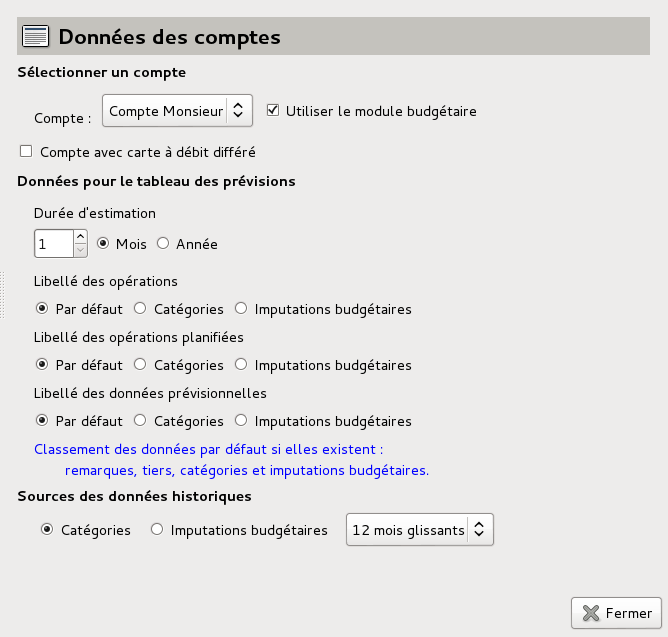
\includegraphics[scale=0.5]{image/screenshot/setup_budget_dataBank}
\end{center}
\caption{Configuration d'un budget pour un compte de banque ou de caisse avec prévisions}
\label{setup_budget_dataBank-img}
\end{figure}
% image centrée
\fi

De plus, dans le pavé des détails du compte concerné, deux nouveaux onglets \menu{Prévisions} et \menu{Données historiques} se sont ajoutés entre les deux autres onglets \menu{Opérations} et \menu{Propriétés}.

% espace pour changement de thème
\vspacepdf{5mm}
Pour configurer les prévisions de ce compte, procédez comme suit :

\begin{enumerate}
	\item ne cochez pas la case de libellé \menu{Compte avec carte à débit différé} ;	 
	\item dans la section \menu{Données pour le tableau des prévisions} saisissez les données :	
		\begin{enumerate}	
			\item définissez la \menu{Durée} : période de temps sur laquelle les prévisions seront calculées, en nombre de mois ou d'années ; elle est au maximum de 5 ans ; 
			\item définissez le \menu{Libellés des opérations} : comment sont décrites les opérations, par une description \menu{Par défaut}, par les \menu{Catégories} ou par les \menu{Imputations budgétaires},
			\item définissez le \menu{Libellés des opérations planifiées} : comment sont décrites les opérations planifiées, par une description \menu{Par défaut}, par les \menu{Catégories} ou par les \menu{Imputations budgétaires},		
			\item définissez le \menu{Libellés des données prévisionnelles} : comment sont décrites les données prévisionnelles, par une description \menu{Par défaut}, par les \menu{Catégories} ou par les \menu{Imputations budgétaires} ; % leave the following line empty to make sure the left alignment of the following note
			
			\vspacehevea{5mm}
			\textbf{Note} : le choix \menu{Par défaut} est le contenu du premier de ces champs pour chaque opération, s'il existe et dans cet ordre : \menu{Remarques}, \menu{Tiers}, \menu{Catégories} et \menu{Imputations budgétaires}.
		\end{enumerate}			
	\item dans la section \menu{Sources des données historiques} :
		\begin{enumerate}	
			\item définissez l'origine des \indexword{données de référence}\index{prévision !données de référence} pour établir les prévisions, grâce à l'un des deux boutons \menu{Catégories} (c'est le choix par défaut) ou \menu{Imputations budgétaires},
			\item définissez la \indexword{période de référence}\index{prévision !période de référence} pour établir les prévisions, grâce à une liste déroulante permettant de choisir soit \menu{12 mois glissants}, soit un exercice, soit un \menu{Nouvel exercice} MAIS UN CLIC DESSUS N'AFFICHE RIEN ???? ; % leave the following line empty to make sure the left alignment of the following note
			
			\vspacehevea{5mm}
			\textbf{Note} : le choix des exercices ne s'affiche que si au moins un exercice a été défini (voir la section \vref{financialyear-start}, \menu{Mise en place des exercices}). % leave the following line empty to make sure the left alignment of the following note
			
			\vspacehevea{5mm}
			\textbf{Note} : ces deux choix peuvent aussi être faits dans l'onglet \menu{Données historiques} du compte concerné.
			\item enregistrez et validez la fenêtre par le bouton \menu{Fermer}, sinon sortez par la touche \key{Échap}.	
		\end{enumerate}
\end{enumerate}

OKOK MAIS PROBLÈME À VOIR CI-DESSUS


\subsubsection{Type compte de caisse\label{setup-budget-data-cash}}

Pour les comptes de caisse, deux cas se présentent, suivant l'état de la case à cocher \menu{Ajouter le tableau des prévisions aux comptes de caisse} (voir la section \vref{setup-budget-general}, \menu{Généralités}) :

\paragraph{Sans prévisions :} si vous n'avez pas coché la case \menu{Ajouter le tableau des prévisions aux comptes de caisse}, une case à cocher et une seule section supplémentaire \ifIllustration s'affichent\refimage{setup_budget_dataCash-img} :
\else s'affichent : 
\fi

\ifIllustration
% image centrée
\begin{figure}[ht]
\begin{center}
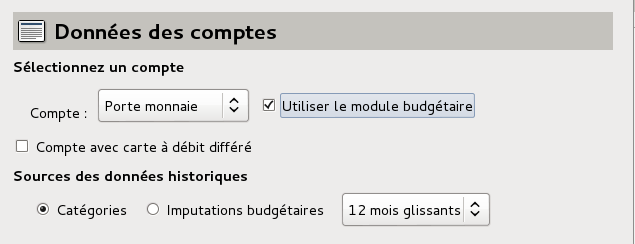
\includegraphics[scale=0.5]{image/screenshot/setup_budget_dataCash}
\end{center}
\caption{Configuration d'un budget pour un compte de caisse sans prévisions}
\label{setup_budget_dataCash-img}
\end{figure}
% image centrée
\fi

\begin{itemize}
	\item une case de libellé \menu{Compte avec carte à débit différé} ; 
	\item une section \menu{Sources des données historiques}.
\end{itemize}

% espace pour changement de thème
\vspacepdf{5mm}   
De plus, dans le pavé des détails du compte concerné, un seul nouvel onglet \menu{Données historiques} s'est ajouté entre les deux autres onglets \menu{Opérations} et \menu{Propriétés} ; 

% espace pour changement de thème
\vspacepdf{5mm}
Pour configurer les prévisions de ce compte, procédez comme suit :
\begin{enumerate}	
	\item définissez l'origine des \indexword{données de référence}\index{prévision !données de référence} pour établir les prévisions, grâce à l'un des deux boutons \menu{Catégories} (c'est le choix par défaut) ou \menu{Imputations budgétaires} ;
	\item définissez la \indexword{période de référence}\index{prévision !période de référence} pour établir les prévisions, grâce à une liste déroulante permettant de choisir soit \menu{12 mois glissants}, soit un exercice, soit un \menu{Nouvel exercice} MAIS UN CLIC DESSUS N'AFFICHE RIEN ???? ; ; % leave the following line empty to make sure the left alignment of the following note
	
	\vspacehevea{5mm}
	\textbf{Note} : le choix des exercices ne s'affiche que si au moins un exercice a été défini (voir la section \vref{financialyear-start}, \menu{Mise en place des exercices}).
	
	\vspacehevea{5mm}
	\textbf{Note} : ces deux choix peuvent aussi être faits dans l'onglet \menu{Données historiques} du compte concerné.
	\item validez la fenêtre par le bouton \menu{Fermer}, sinon par la touche \key{Échap}.	
\end{enumerate}

OKOK MAIS PROBLÈME À VOIR CI-DESSUS

\paragraph{Avec prévisions :}si vous avez coché la case \menu{Ajouter le tableau des prévisions aux comptes de caisse}, une case à cocher et deux sections supplémentaires \ifIllustration s'affichent\refimage{setup_budget_dataBank-img} :
\else s'affichent : 
\fi

\begin{itemize}
	\item une case de libellé \menu{Compte avec carte à débit différé} ; 
	\item une section \menu{Données pour le tableau des prévisions}, seulement si vous avez coché la case \menu{Ajouter le tableau des prévisions aux comptes de caisse} ; 
	\item une section \menu{Sources des données historiques}.
\end{itemize}

% espace pour changement de thème
\vspacepdf{5mm}
De plus, dans le pavé des détails du compte concerné, deux nouveaux onglets \menu{Prévisions} et \menu{Données historiques} se sont ajoutés entre les deux autres onglets \menu{Opérations} et \menu{Propriétés}.

% espace pour changement de thème
\vspacepdf{5mm}
La configuration des prévisions de ce compte se fait de la même manière que pour les comptes bancaires (voir le paragraphe \vref{setup-budget-data-bank}, \menu{Type compte bancaire}).



\subsubsection{Type compte de passif avec carte bancaire à débit différé\label{setup-budget-data-liabilityWithCard}}

Pour ces comptes, la fenêtre de configuration est la même que pour un compte de caisse, elle se configure de la même manière, et le pavé des détails affiche les mêmes onglets (voir le paragraphe \vref{setup-budget-data-cash} \menu{Type compte de caisse}, \menu{Sans prévisions}).

\ifIllustration
% espace pour lien hypertexte solidaire
\newpage
\fi


\subsubsection{Type compte bancaire avec carte bancaire à débit différé\label{setup-budget-data-bankWithCard}}

Pour ces comptes, la fenêtre de configuration est la même que pour un compte bancaire, elle se configure de la même manière, et le pavé des détails affiche les mêmes onglets (voir le paragraphe \vref{setup-budget-data-bank}, \menu{Type compte bancaire}).


\subsubsection{Type compte de caisse avec carte bancaire à débit différé\label{setup-budget-data-cashWithCard}}

Cette possibilité permet d'établir des prévisions sur ce type de compte auquel pourrait être dédiée une carte bancaire, qui pourrait être par exemple un porte-monnaie électronique à débit différé, si cela existe, ou toute autre utilisation dont vous pourriez avoir besoin.

% espace pour changement de thème
\vspacepdf{5mm}
Pour les comptes de caisse, deux cas se présentent, suivant l'état de la case à cocher   \menu{Ajouter le tableau des prévisions aux comptes de caisse} (voir la section \vref{setup-budget-general}, \menu{Généralités}) :

\paragraph{Sans prévisions :} si vous n'avez pas coché la case \menu{Ajouter le tableau des prévisions aux comptes de caisse}, la fenêtre de configuration est la même que pour un compte de caisse sans prévisions, elle se configure de la même manière, et le pavé des détails affiche les mêmes onglets (voir le paragraphe \vref{setup-budget-data-cash}, \menu{Type compte de caisse}, \menu{Sans prévisions}).

\paragraph{Avec prévisions :} si vous avez coché la case \menu{Ajouter le tableau des prévisions aux comptes de caisse}, la fenêtre de configuration est la même que pour un compte bancaire, elle se configure de la même manière, et le pavé des détails affiche les mêmes onglets (voir le paragraphe \vref{setup-budget-data-bank}, \menu{Type compte bancaire}).


\subsubsection{Type compte d'actif\label{setup-budget-data-asset}}

Il n'y a pas de module budgétaire pour un compte d'actif, on ne peut donc pas le valider.



